\documentclass{report}
\usepackage[spanish]{babel}
\usepackage{url}
\usepackage[titletoc,toc,title]{appendix}
\usepackage{amsmath}
\usepackage{amsthm}
\usepackage{amssymb}
\usepackage[letterpaper, top=30mm, bottom=30mm, left=30mm, right=30mm]{geometry}
\usepackage[T1]{fontenc}
\usepackage[sort]{natbib}
\usepackage{libertine}
\renewcommand*\familydefault{\sfdefault} 
\usepackage{hyperref}
\usepackage{floatflt}
\usepackage{graphicx}

\setlength{\parindent}{0pt}
\setlength{\parskip}{1em}

\makeatletter
\providecommand*{\diff}%
        {\@ifnextchar^{\DIfF}{\DIfF^{}}}
\def\DIfF^#1{%
        \mathop{\mathrm{\mathstrut d}}%
                \nolimits^{#1}\gobblespace
}
\def\gobblespace{%
        \futurelet\diffarg\opspace}
\def\opspace{%
        \let\DiffSpace\!%
        \ifx\diffarg(%
                \let\DiffSpace\relax
        \else
                \ifx\diffarg\[%
                        \let\DiffSpace\relax
                \else
                        \ifx\diffarg\{%
                                \let\DiffSpace\relax
                        \fi\fi\fi\DiffSpace} 

\author{Claude E. Shannon}
\title{Una teor\'{\i}a matem\'{a}tica de la comunicaci\'{o}n}
\date{1948}
\begin{document}
\maketitle

\newtheorem{theorem}{Teorema}[section]
\newtheorem{definition}{Definici\'{o}n}[section]

\begin{abstract}
  Esta es una traducci\'{o}n al espa\~{n}ol del art\'{\i}culo
  publicado por Shannon en {\em The Bell System Technical Journal},
  realizado a base del PDF disponible en
  \url{http://cm.bell-labs.com/cm/ms/what/shannonday/shannon1948.pdf}
  como un esfuerzo colectivo de estudiantes de octavo semestre del ITS
  de la FIME de la UANL por puntos extra en la unidad de apxrendizaje
  {\em Teor\'{\i}a de la informaci\'{o}n y m\'{e}todos de
    codificaci\'{o}n}, impartida por Dra.\ Elisa Schaeffer en la
  primavera del 2013.
\end{abstract}

\documentclass{article}
\title{Cartesian closed categories and the price of eggs}
\author{Jane Doe}
\date{September 1994}
\begin{document}
   \maketitle
   Hello world!
\end{document}
 % pp. 1--3 recientemente confirmados
En caso de que existan restricciones en secuencias permitidas todav\'ia se puede 
obtener una ecuaci\'on diferencial de este tipo y encontrar C de la ecuaci\'on 
caracter\'istica. En el caso mencionado anteriormente de la telegraf\'ia

$N(t) = N(t-2)+N(t-4)+N(t-5)+N(t-7)+N(t-8)+N(t-10)$

como se ve por el c\'alculo de secuencia de los s\'imbolos de acuerdo al \'ultimo o 
al siguiente \'ultimo s\'imbolo ocurriendo.
Por lo tanto $-log\mu_{0}$ donde $\mu_{0}$ es la ra\'iz positiva de 
$1 = \mu^{2}+\mu^{4}+\mu^{5}+\mu^{7}+\mu^{8}+\mu^{10}$. Resoviendo eso encontramos 
que $C = 0.539$.

Una restricci\'on general se puede colocar en secuencias como la siguiente: Imagenemos
un numero de estados posibles $a_{1}, a_{2},...,a_{m}$. Por cada estado solo 
ciertos s\'imbolos del conjunto $S_{1},...S_{n}$ pueden ser transmitidos 
(diferentes subconjuntos por cada estado). Cuando uno de esos han sido transmitidos 
el estado cambia a un nuevo estado dependiendo de el viejo estado y del s\'imbolo en 
particular transmitido. Un ejemplo simple de esto es el caso del tel\'egrafo. Hay 
dos estados en funci\'on de si o no un espacio era el \'ultimo s\'imbolo transmtido. 
Si es as\'i, entonces s\'olo un punto o una raya puede ser enviado al lado y el 
estado cambia siempre. Si no, cualquier s\'imbolo puede ser transmitido y los 
cambios de estado si un espacio es enviado, de lo contrario sigue siendo el mismo. 
Las condiciones pueden ser indicadas en una gr\'afica lineal como se ve en la 
figura 2. Los puntos de uni\'on correspoden a los 


estados y las l\'ineas indicando los s\'imbolos posibles en un estado y el estado resultante. 
En el Ap\'endice 1 se muestran que si las condiciones en las secuencias 
permitidas puede ser descrita en la forma C puede existir y se puede calcular de 
acuerdo con el siguiente resultado:
\begin{theorem} Siendo $b_{ij}^{(s)}$ la duraci\'on del s\'imbolo $s^{th}$ el cual 
es permisible en el estado i y conduce al estado j. Despu\'es la capacidad del canal 
C es igual a $logW$ donde $W$ es la ra\'iz real m\'as larga de la ecuaci\'on:
\begin{equation}
\left|\sum_{s}W^{-b_{ij}^{(s)}}-\delta_{ij}\right|=0
\end{equation}
donde $\delta_{ij}=1 si i=j$ y es cero en cualquier otro caso
\end{theorem}
Por ejemplo en el caso del tel\'egrafo el determinante es:
\begin{equation}
\begin{vmatrix}
-1&(W^{-2}+W^{-2}) \\ 
 (W^{-3}+W^{-6})&(W^{-2}+W^{-2}-1) 
\end{vmatrix}=0
\end{equation}
Esta expansi\'on conduce a la ecuaci\'on dada anteriormente para este caso.

\section{LA FUENTE DISCRETA DE LA INFORMACI\'ON}
Hemos visto que bajo condiciones muy generales el logaritmo del n\'umero de se\~nales 
posibles en un canal discreto aumenta linealmente con el tiempo. La capacidad de 
transmisi\'on de informaci\'on se puede especificar dando a esta tasa de aumento, el n\'umero 
de bits por segundo necesarios para especificar la se\~nal particular utilizada.
Consideremos ahora la fuente de informaci\'on. ?`C\'omo es una fuente de informaci\'on a ser 
descrita matem\'aticamente, y la cantidad de informaci\'on en bits por segundo se produce en una 
fuente dada? El principal punto en cuesti\'on es la efecto de los datos estad\'isticos sobre la 
fuente en la reducci\'on de la capacidad requerida de la canal, por el uso de una correcta 
codificaci\'on de la informaci\'on. En la telegraf\'ia, por ejemplo, los mensajes para ser 
transmitidos consisten en secuencias de letras. Estas secuencias, sin embargo, no son 
completamente aleatorias. En general, las oraciones tienen una estructura estad\'istica de, 
por ejemplo, Ingl\'es. La letra E se produce con m\'as frecuencia que Q, la secuencia TH con m\'as 
frecuencia que XP, etc. La existencia de esta estructura permite hacer un ahorro en el tiempo (o 
capacidad de canal) para codificar correctamente las secuencias de mensajes en una secuencia 
de se\~nales. Esto ya se hace en una medida limitada en telegraf\'ia utilizando el s\'imbolo de canal 
m\'as corto, un punto, por la m\'as letra E que es la m\'as com\'un en Ingl\'es, mientras que las letras infrecuentes, 
Q, X, Z est\'an representados por secuencias m\'as largas de puntos y rayas. esta idea se lleva a\'un 
m\'as lejos en ciertos c\'odigos comerciales donde las palabras y frases comunes est\'an representados
por cuatro o cinco grupos de c\'odigo de letra con un considerable ahorro de tiempo promedio. 
Los telegramas est\'andar de saludo y aniversario se han usado tanto hasta el punto de 
que se codifican una o dos frases en una secuencia relativamente corta de n\'umeros.

Podemos pensar en una fuente discreta de generar el mensaje, s\'imbolo por s\'imbolo. Se elegir\'a 
una sucesi\'on de s\'imbolos de acuerdo con ciertas probabilidades dependiendo, en general, 
de las opciones anteriores, as\'i como los s\'imbolos en cuesti\'on. Un sistema f\'isico, o 
un modelo matem\'atico de un sistema que produce una secuencia de s\'imbolos gobernadas por un 
conjunto de probabilidades, se le conoce como un proceso estoc\'astico. 
Podemos considerar por lo tanto que una fuente discreta puede ser representada por un proceso 
estoc\'astico. A la inversa, cualquier proceso estoc\'astico que produce una secuencia discreta 
de s\'imbolos elegidos a partir de un conjunto finito puede ser 
considerado una fuente discreta. Esto incluye casos como:

\begin{enumerate}
\item Idiomas naturales escritos como el Ingl\'es, Alem\'an y Chino.
\item Fuentes de informaci\'on continuos que se han vuelto discreta por alg\'un proceso 
de cuantificaci\'on. Por ejemplo, la se\~nal de voz cuantizada desde un transmisor PCM, o 
una se\~nal de televisi\'on cuantizada.
\item Casos matem\'aticos en los que simplemente se definen abstractamente procesos estoc\'asticos 
que generan una secuencia de s\'imbolos. Los siguientes son ejemplos de este \'ultimo tipo de fuente.
\begin{enumerate}
\item Supongamos que tenemos cinco letras A, B, C, D, E, que se eligen cada una con probabilidad 0.2, 
elecciones sucesivas siendo independientes. Esto dar\'ia lugar a una secuencia, la siguiente 
es un t\'ipico ejemplo.

B D C B C E C C C A D C B D D A A E C E E A

A B B A E D E C A C E E E E B A C B C E A D

Este fue construido con el uso de una tabla de azar.
\item Utilizando las mismas cinco letras y siendo las probabilidades 0.4, 0.1, 
0.2, 0.2, 0.1, respectivamente, con decisiones independientes sucesivas. Un mensaje 
t\'ipico de esta fuente es entonces:

A A A C D C B D C E A A D A D A C E D A

E A D C A B E D A D E D C C A A A A A D.

\item Una estructura m\'as complicada se obtiene si los s\'imbolos no son elegidos 
de manera independiente pero sus probabilidades dependen de las letras anteriores. En 
el caso m\'as simple este tipo de elecci\'on depende solamente de la letra anterior y no
de las que estan antes. La estructura estad\'istica puede entonces ser descrita por un 
conjunto de probabilidades de transici\'on $p_{i}(j)$, la probabilidad de que la letra `$i$ 
es seguida por la letra $j$. Los \'indices de $i$ y $j$ se extienden sobre todos los 
s\'imbolos posibles. Una segunda manera equivalente de especificar la estructura es dar 
el "diagrama" de probabilidades $p(i,j)$, la frecuencia relativa de el diagrama $i j$.
La frecuencia de letras $p(i)$, (la probabilidad de la letra i), la transici\'on de 
probabilidades $p_{i}(j)$ y el diagrama de probabilidades $p(i,j)$ son descritos en las 
siguientes formulas:
\begin{equation}
p(i)=\sum_{j}p(i,j)=\sum_{j}p(j,i)=\sum_{j}p(j)p_{j}(i) 
\end{equation}
\end{enumerate}
\end{enumerate}
 % pp. 4--5 recientemente asignados
4. Representacion grafica de procesos Markovianos

Los procesos estocasticos del tipo descrito arriba son matematicamente conocidos como Procesos Markovianos Discretos y han sido estudiados extensivamente en la literatura.^{6} El caso general puede ser descrito de la siguiente manera: Existe un numero finito de posibles "estados" de un sistema; S_{1}, S_{2}, ...,S_{n}. Adem\'{a}s existen un conjunto de probabilidades de transicion; p_{i}(j) la probabilidad que si el sistema esta en estado S_{i} entonces enseguida vaya al estado S_{j}. Para realizar este proceso Markoviano en una fuente de información solo necesitamos asumir que una letra es producida para cada transicion desde un estado a otro. Los estados corresponderán al ``residuo de influencia'' de letras precedentes. \\
La situacion puede ser representada graficamente como se muestra en las figuras 3, 4 y 5. Los "estados" son los puntos de union

% aqui va figura 3

en la grafica y las probabilidades y letras son producidas para una transicion son dadas ademas de la linea correspondiente. La figura 3 es para el ejemplo B en la seccion 2, mientras que la figura 4 corresponde al ejemplo C. En la figura 3

%figura 4

solamente hay un estado ya que letras sucesivas son independientes. En la figura 4 hay tantos estados como letras. \newline
Si un ejemplo de un triagrama fuera construido, habr\'{i}a por maximo n^{2} estados correspondiendo a los posibles pares de letras precediendo a uno que haya sido elegido. La figura 5 es un grafo para el caso de estructura de palabras en el ejemplo D. Aqui S corresponde a el simbolo ``espacio''. \newline

5. Fuentes erg\'{o}dicas y mixtas.

Como se ha indicado anteriormente, una fuente discreta para nuestros propositos puede ser considerada representada por un proceso Markoviano. Entre los posibles procesos discretos Markovianos existe un grupo con propiedades especiales con importancia en la teoria de la comunicacion. Esta clase especial consiste en los procesos ``ergodicos'' y deberiamos de llamar a las fuentes correspondientes, fuentes ergodicas. Aunque una definicion rigurosa de los procesos ergodicos es algo complicada, la idea general es simple. En un proceso ergodico cada secuencia producida por el proceso permanece igual en sus propiedades estadisticas. Por lo tanto las frecuencias de letras, las frecuencias de bigramas, etc., obtenidos de una secuencia en particulas, se acercaran a un limite definido conforme la longitud de las secuencua aumenta, independientemente de la secuencia en particular. En realidad esto no es meramente cierto para cada secuencia pero el grupo para el cual esto es falso tiene una probabilidad de cero. Practicamente, la propiedad ergodica significa homogeneidad estadistica. \\
Todos los ejemplos de lenguaje artificial dados anteriormente son ergodicos. Esta propiedad está relacionada a la estructura de los grafos correspondientes. Si el grafo tiene las siguientes dos propiedades el proceso correspondiente será ergodico:

\begin{enumerate}
   \item El grafo no consiste de dos partes aisladas A y B dado que es imposible ir desde los puntos de union en la parte A a los puntos de union en la parte B a traves de las lineas del grafo en la direccion de las flechas y tambien es imposible ir desde las uniones en la parte B a las uniones en la parte A. 
   \item 
\end{enumerate}

\begin{equation}
b = a - 2
\end{equation}
 % pp. 7--14 recientemente confirmados
\chapter{Representaci\'{o}n de las operaciones de codificaci\'{o}n y decodificaci\'{o}n}
\label{sec:8}

A\'{u}n tenemos que representar matem\'{a}ticamente las operaciones realizadas por el transmisor y el receptor en la informaci\'{o}n codificada y decodificada. Cualquiera de estos se llama transductor discreto. La entrada al transductor es una secuencia de s\'{i}mbolos de entrada y su salida una secuencia de s\'{i}mbolos de salida. El transductor puede tener una memoria interna de modo que su salida depende no s\'{o}lo del s\'{i}mbolo actual de entrada, sino tambi\'{e}n de su historial anterior. Se supone que la memoria interna es finito, es decir, existe un n\'{u}mero finito m de posibles estados del transductor y que su salida es una funci\'{o}n del estado actual y el s\'{i}mbolo de entrada presente. El estado siguiente ser\'{a} una funci\'{o}n segunda de estas dos cantidades. As\'{i}, un transductor puede ser descrito por dos funciones:
\begin{equation}y_{n}= f\left ( x_{n}, \alpha_{n} \right )\end{equation}
\begin{equation}\alpha_{n+1} = g\left ( x_{n}, \alpha_{n} \right )\end{equation}
Donde

$x_{n}$ es el n^{esimo} s\'{i}mbolo de entrada,

$\alpha_{n}$ es el estado del transductor cuando el n^{esimo} s\'{i}mbolo de entrada es introducido,

$y_{n}$ es el s\'{i}mbolo de salida \left ( o la secuencia de s\'{i}mbolos de salida \right ) producida cuando x_{n} es introducida si el estado de is \alpha_{n}.

Si el s\'{i}mbolo de salida es un transductor puede ser identificado con un s\'{i}mbolo de entrada de un segundo, se pueden conectar en t\'{a}ndem y el resultado es tambi\'{e}n un transductor. Si existe un segundo transfuctor que opera sobre la salida de la primera y recupera el original de entrada, el primer tranductor se llama no singular y el segundo es llamado el inverso.

\begin{theorem}
\label{th:7}
La salida de un transductor de estado finito accionado por una fuente de estado finito estad\'{i}stica es una fuente de estado finito estadi\'{i}stica, con la entrop\'{i}a \left (por unidad de tiempo \right) menor o igual a la de la entrada. Si el transductor es no singular son iguales.\end{theorem}

Sea $\alpha$ el estado de la fuente, que produce una secuencia de s\'{i}mbolos $x_{i}$; y sea $\beta$ el estado del transductor, que produce, en su salida, bloques de s\'{i}mbolos $y_{j}$. El sistema combinado puede ser representado por el espacio del producto de los pares $\left ( \alpha, \beta \right )$. Dos puntos en el espacio $\left ( \alpha_{1}, \beta_{1} \right )$ y $\left ( \alpha_{2}, \beta_{2} \right )$, son conectados por una linea si $\alpha{1}$ puede producir una $x$ que cambie $\beta_{1}$ a $\beta_{2}$, y esta linea es dada por la probabilidad de $x$ en este caso. La linea es etiquetada con el bloque de s\'{i}mbolos $y_{j}$ producida por el transductor. La entropia de la salida puede ser calculada con el peso de la sumas de los estados. Si sumamos primero cada $\beta$ resultante es menor o igual que el termino correspondiente a $\alpha$, por lo tanto la entropia no es incrementada. Si el tranductor es no singular sea su salida conectada al transuduct inverso. Si $H_{'}^{1}$, $H_{'}^{2}$ y $H_{'}^{3}$ son las salidas de las entropias de la fuente, el primero y el segundo transductor respectivamente, entonces $H_{'}^{1}\geqH_{'}^{2}\geqH_{'}^{3}=H_{'}^{1}$ por lo tanto $H_{'}^{1}=H_{'}^{2}$.

Supongamos que tenemos un sistema de restricciones sobre las posibles secuencias del tipo que puede ser representado por grafo lineal como en la Fig. 2. Si las probabilidades $p_{ij}^{(s)}$ son asignados por varias lineas conectadas estado $i$ al estado $j$ se convertir\'{i}a en una fuente. Hay una asignaci\'{o}n particular que maximiza la entrop\'{i}a resultante (v\'{e}ase Ap\'{e}ndice 4).

\begin{theorem}
\label{th:8}
Sea el sistema de restricciones considerado como canal tiene una capacidad $C = logW$. Si se asigna.} $\begin{equation} P_{ij}^{(s)} = \frac{B_{j}}{B_{i}}W^{-\iota_{ij}^{(s)}} \end{equation}$ \textit{donde $\iota_{ij}^{(s)}$ es la duraci\'{o}n del s^{esimo} s\'{i}mbolo que va desde el estado $i$ hasta el estado $j$ y satisfaciendo $B_{i}$} $\begin{equation} B_{i}=\sum_{s.j} B{j}W^{-\iota_{ij}^{(s)}} \end{equation}$ \textit{entonces $H$ es maximizada e igual a C.
\end{theorem}

Por asignaci\'{o}n correcta de las probabilidades de transici\'{o}n de la entrop\'{i}a de los s\'{i}mbolos en un canal puede ser maximizada a la capacidad del canal. 

\clearpage

\chapter{El teorema fundamental de un canal sin ruido}
\label{sec:9}

FALTA

\begin{theorem}
\label{th:9}
Que una fuente tenga entropia $H$...
\end{theorem}

\clearpage

\chapter{Discusi\'{o}n y ejemplos}
\label{sec:19}

FALTA
 % pp. 15--18 recientemente asignados
Este doble proceso puede decodificar el mensaje original en los mismo s\'{i}mbolos, pero con un radio de compresi\'{o}n promedio de $\frac{7}{8}$.

Como un segundo ejemplo considere una fuente que produce una secuencia de A's y B's con probabilidad p para A y q por B. Si p << q tenemos que

\begin{equation}
H = - log p^p (1 - p)^1^-^p
= -p log p(1-p)^(^1^-^p^)^/^p
= p log \frac{e}{p}
\end{equation}

En tal caso uno puede construir una codificaci\'{o}n del mensaje sobre un canal de 0, 1 lo suficientemente buena mediante el env\'{i}o de una secuencia especial, por ejemplo 0000, para el s\'{i}mbolo poco frecuente A y a continuaci\'{o}n, una secuencia indicando el n\'{u}mero siguiente de B's. Esto podr\'{i}a ser indicado por una representaci\'{o}n binaria con todos los n\'{u}meros que contienen la secuencia especial eliminada. Todos los n\'{u}meros hasta el 16 son representados como de costumbre; el 16 es representado por el siguiente n\'{u}mero binario despues de 16 que no contiene 4 ceros, es decir, 17  = 10001, etc.

Se puede demostrar que a medida que $p\rightarrow{0}$ los enfoques de codificaci\'{o}n ideales proporcionan la longitud de la secuencia especial es ajustada correctamente.

\part{El canal discreto con ruido}
\label{part:2}

\chapter{Representaci\'{o}n de un canal discreto con ruido}
\label{sec:11}

Ahora consideremos el caso en donde la señal es perturbada por ruido durante la transmisi\'{o} o en algunas de las terminales. Esto significa que la señal recibida no es necesariamente el mismo que el enviado por el transmisor. Dos casos pueden ser distinguidos. Si una señal particular transmitida siempre produce la misma señal recibida, es decir, la señar recibida es una funcion definida de la señal transmitida, entonces el efecto puede ser llamado distorsi\'{o}n. Si la función tiene inversa -las dos señales transmitidas no deben de producir la misma señal recibida- la distorsi\'{o} puede ser corregida, al menos al principio, solamente por la realizaci\'{o}n de la operaci\'{o}n de la funci\'{o}n inversa de la señal recibida.

El caso de inter\'{e}s aqu\'{i} es aquel en el que la señal no siempre se someta al mismo cambio en la transmisi\'{o}n. En este caso podemos asumir que la señal recibida E es una funci\'{o} de la señal de transmisi\'{o}n S y una segunda variable, el ruido N.

\begin{equation}
E = f\left (S,\right N)
\end{equation}

El ruido es considerado como una variable de probabilidad igual al mensaje que estaba por encima. En general, esto puede ser representado como un proceso estoc\'{a}stico adecuado. El tipo m\'{a}s general de canales discretos con ruido que consideramos es una generalizaci\'{o}n de el canal libre de ruido de estado finito descrito anteriormente. Podemos asumir un n\'{u}mero finito de estados y un conjunto de probabilidades

\begin{equation}
P_{\alpha, i}\left ( \beta , \right j).
\end{equation}

Esta es la probabilidad, si el canal est\'{a} en el estado $\alpha$ y el s\'{i}mbolo $i$ es transmitido, el s\'{i}mbolo $j$ sera recibido y el canal se queda en estado $\beta$. As\'{i} $\alpha$ y el rango de $\beta$ sobre las posibles señales recibidas. En el caso de que los s\'{i}mbolos sucesivos son perturbados de forma independiente por el ruido solo hay un estado, y el canal es descrito por el conjunto de probablidades de transici\'{o}n $P_{i}\left (j\right)$, la probabilidad de transmitir un s\'{i}mbolo $i$ sera recibido como $j$·

Si el canal con ruido es alimentado por una fuente hay dos procesos en trabajo: la fuente y el ruido. Por lo tanto hay un n\'{u}mero de entrop\'{i}as que se pueden calcular. En primer lugar est\'{a} la entrop\'{i}a $H(x)$ de la fuente o de la entrada al canal (\'{e}stos ser\'{a}n iguales si el transmisor es no singular). La entrop\'{i}a de la salidad del canal, es decir, la señal recibida se denota por $H(y)$. En el caso sin ruido $H(y) = H(x)$. El conjunto de entrop\'{i}as de entrada y salida ser\'{a} $H\left(x\right y)$. Finalmente donde haya dos entrop\'{i}as condicionales $H_{x}(y)$ y $H_{y}(x)$, la entrop\'{i}a de la salida cuando la entrada es conocida y a la inversa. Entre esas cantidades tenemos las relaciones

\begin{equation}
H\left (x,\right y) = H(x) + H_{x}(y) = H(y) + H_{y}(x).
\end{equation}

Todas estas entrop\'{i}as se pueden medir en funci\'{o}n de por segundo o en funci\'{o}n de cada s\'{i}mbolo.

\clearpage

\chapter{Equivocaci\'{o}n y capacidad de canal}
\label{sec:12}

Si el canal es con ruido por lo general no es posible el reconstruir el mensaje original o la señal transmitida con certeza por cualquier operaci\'{o} efectuada sobre la señal recibida $E$. Hay, sin embargo, maneras de transmitir la informaci\'{o}n que son \'{o}ptimas en el combate contra el ruido. Este es el problema que consideramos ahora

Supongamos que hay dos posibles s\'{i}mbolos 0 y 1, y estamos transmitiendo a una velocidad de 1000 s\'{i}mbolos por segundo con probabilidad de $p_{0} = p_{1} = \frac{1}{2}$. Por lo tanto nuestra fuenta est\'{a} produciendo informaci\'{o}n a la velocidad de 1000 bits por segundo. Durante la transmisi\'{o}n del ruido se introduce errores de manera que, en promedio, 1 en 100 se recibieron incorrectamente (un 0 como 1, o 1 como 0). ¿Cu\'{a}l es la tasa de transmisi\'{o}n de informaci\'{o}n? Ciertamenet menos de 1000 bits por segundo aproximadamente el 1\% de los s\'{i}mbolos recibidos son correctos. Nuesto primer impulso podr\'{i}a decir que la tasa es de 990 bits por segundo, simplemente el n\'{u}mero de errores esperados. Esto no es satisfactorio ya que no se tiene en cuenta la falta de conocimiento de d\'{o}nde se producen los errores del destinatario. Es posible llevarlo a un caso extremo y supongamos que el ruido es tan grande que los s\'{i}mbolos recibidos son totalmente independientes de los s\'{i}mbolos transmitidos. La probalidad de recibir $1$ es $\frac{1}{2}$ en todo lo que se transmite y de manera similar para 0. Luego, alrededor de la mitada de los s\'{i}mbolos recibidos son correctos debido al azar, y nos estar\'{i} dando el cr\'{e}dito del sistema para la transmisi\'{o}n de 500 bits por segundo, cuando en realidad la informaci\'{o} no se transmite en absoluto. Igualmente la transmisi\'{o}n "correcta" se obtendr\'{i}a mediante la dispensaci\'{o}n con el canal entero y lanzando una moneda en el punto de recepci\'{o}n.

FALTA

\begin{theorem}
\label{th:10}
Si el canal de correcci\'{o}n...
\end{theorem}

FALTA

\begin{figure}[!ht]
\centerline{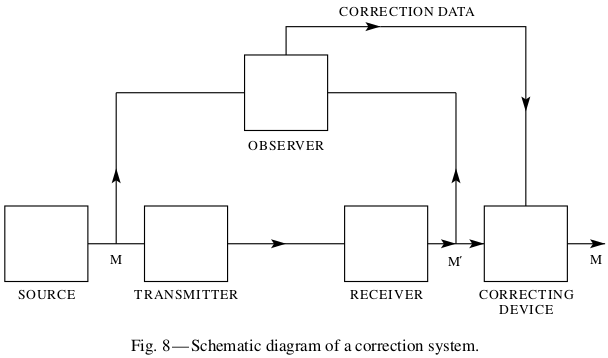
\includegraphics[width=120mm]{Imagenes/Pagina21-Figura8.png}}
\caption{Un diagrama esquem\'{a}tico de un sistema de correcci\'{o}n.}
\label{fig:8}
\end{figure}

FALTA

\begin{exmp}
Suponga que los errores suceden al azar...
\end{exmp}

FALTA

\begin{theorem}
\label{th:11}
Que un canal discreto tenga
\end{theorem}

FALTA

\clearpage

\chapter{El teorema fundamental para un canal discreto con ruido}
\label{sec:13}

\begin{figure}[!ht]
\centerline{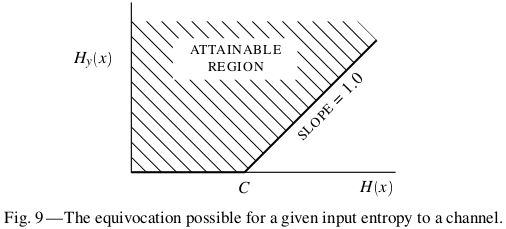
\includegraphics[width=100mm]{Imagenes/Pagina22-Figura9.png}}
\caption{La equivocaci\'{o}n posible para una entropia de entrada dada
  a un canal.}
\label{fig:9}
\end{figure}

FALTA

\begin{figure}[!ht]
\centerline{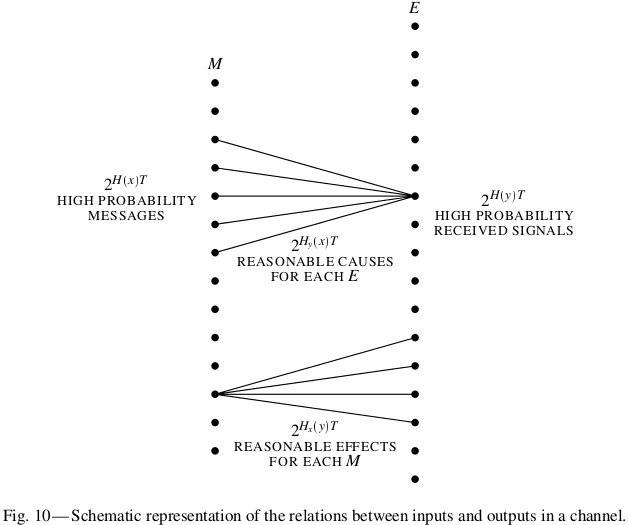
\includegraphics[width=140mm]{Imagenes/Pagina23-Figura10.png}}
\caption{Una representaci\'{o}n esquem\'{a}tica de las relaciones
  entre las entradas y salidas en un canal.}
\label{fig:10}
\end{figure}

FALTA

\clearpage

\chapter{Discussion}
\label{sec:14}

FALTA

 % pp. 19--25 recientemente confirmados
En el caso sin ruido un retraso generalmente requiere para la codificacion\'on ideal ahora 
esta tiene una funci\'on adicional que permite una muestra larga de ruido para afectar la señal antes de un juicio, se hace 
en el punto de resepci\'on  para el mensaje original.Incrementando el tamaño del ejemplo siempre agudiza las posibles afirmaciones estadisticas.

El contenido del teorema 11 y su prueba se pueden formular de una manera diferente que muestra 
una conexi\'on sin ruido de una manera mas clara.Considere las posibles duraciones de las señales T y supongamos 
un subconjutno de ellos se seleccionan para ser usados. Los que esten en el subconjunto se utilizen todos con igual probabilidad, y suponiendo 
que el resector es construido para seleccionar, como la señal original. la causa mas probable de subconjutno cuando 
una señal perturbada es recivida.Nosotros definimos \begin{em}N(T,q)\end{em} siendo el numero maximo de señales que podemos elegir para el subconjunto tal que la probabilidad de una interpretaci\on incorrecta sea menor o igual a q.

\begin{em}Teorema 12:\end{em} \displaystyle\lim_{t \to{}\infty}\frac{\log{N}(T,q)}{T} = C \begin{em}, Donde C es la capacidad de canal,a condici\'on que q no sea igual a 0 o 1\end{em}

En otras palabras, no importa lo que nos propusimos de limites de confiabilidad, podemos distinguir de forma fiable en el tiempo T 
suficientes mensajes para corresponder a CT bits, cuando T es suficientemente grande. En el teorema 12 podemos comparar 
la capacidad de un canal sin ruido en la secci\'on uno.

\begin{center}
EJEMPLO DE UN CANAL DISCRETO Y SU CAPACIDAD
\end{center} 

Un ejemplo simple de un canal discreto se indica en la figura 11.Hay tres posibles simbolos. EL primero 
nunca se vera afectado por el ruido.El segundo y la tercera tiene cada una probabilidad p de que viene a trav\'es impertubable q de ser cambiado en el otro elemto par.Nosotros tenemos (dejar =  \alpha = -[plogp + q\log{q}] y p y q son probabilidades de estar usando los simbolos primero y segundo).

\begin{centerMe gusta ·  · Compartir · Hace 9 minutos · }
H(x) = -P\log{P} - 2Q\log{Q}
H_y(x) = 2Q\alpha
\end{center}


Nosotros deseamos elegir P y Q, de tal manera que se maximice H(x) - H_y(x) sujeto a la restricci\'on P + 2Q = 1. 

Por lo tanto concideremos:

\begin{center}
U = -P\log{P} - 2Q\log{Q} -2Q\alfa + \lambda(P+2Q)

\frac{{\partial U}}{{\partial P}} = -1 - \log{P} + \lambda = 0

\frac{{\partial U}}{{\partial P}} = -2 - 2\log{Q} -2\alpha + 2\lambda = 0
\end{center}


Eliminando \lamda

\begin{center}
\log{P} = \log{Q} + \alpha
P = Q e^\alpha = Q\beta 
\end{center}

\begin{center}
P = \frac{\beta}{\beta + 2}   Q = \frac{1}{\beta + 2}
\end{center}

La capacidad del canal es de:

\begin{center}
C = \log{\frac{\beta + 2}{\beta}}
\end{center}

Notese como esto comprueba los valores obvios en los casos: p = 1 y p = \frac{1}{2}. En primero, \beta = 1 y C = \log{3}, el cual es correcto debido a que el canal es entonces sin ruido con tres posibles s\'imbolos. Si p = \frac{1}{2}, \beta = 2 y C = \log{2}.Aqu\'i el segundo y el tercer s\'imbolos, no se pueden distinguir en absoluto y act\'uan conjuntamente como un solo s\'imbolo. El primer simbolo se utiliza con una probabilidad P = \frac{1}{2}  y el segundo junto al tercero con probabilidad \frac{1}{2}.Esto puede ser distribuido entre ellos de cualquier modo deseado y todav\'ia alcanzar la m\'axima capacidad.
Para los valores intermedios de la capacidad del canal p estara entre \log{2} y \log{3}.Esta distinci\'on 
entre el segundo y tercer s\'imbolo transmite alguna informaci\'on, pero no tanto como en el caso sin ruido.

El primer s\'imbolo se utiliza tanto mas frecuentemente que los otros dos, debido a su ausencia de ruido.

\begin{center}
16. LA CAPACIDAD DE CANALES EN CIERTOS CASOS ESPECIALES
\end{center}

Si el ruido afecta símbolos sucesivos de canal de forma independiente pueden ser descritos por un conjunto de transici\'on de probabilidades p_{i,j}.Esta es la probabilidad, si el simbolo i es enviado, que j sera recibido.La tasa de canal maximo viene dado por el m\'aximo de

\begin{center}
- \sum_{i,j}P_i p_{i,j} \log{\sum{P_i p_{i,j}}} + \sum_{i,j}P_i p_{i,j}\log{p_{i,j}}
\end{center}
 
Multiplicar por P_s y sumando en s muestra que \mu = C. Vamos a la inversa de p_{sj} (si existe) en h_{st}  de modo que \sum_{s} h_{st} p_{sj} = \delta_{tj}.Entonces: 

\begin{center}
\sum_{s,j}h_{st} p_{s,j} \log{p_{s.j}} - \log{\sum_{i}P_i p_{i,t}} = C \sum_{s} h_{s,t}
\end{center}
Por lo tanto:

\begin{center}
\sum_{i} P_i p_{i,t} = exp[- C \sum_{s} h_{s,t}+ \sum_{s,j} h_{s,t} p_{s,j} \log{p_{s,j}}]
\end{center}

o:  
\begin{center}
P_i = \sum_{t} h_{i,t} exp[ - C \sum_{s} h_{s,t}+ \sum_{s,j} h_{s,t} p_{s,j} \log{p_{s,j}} ]
\end{center}


Este es el sistema de ecuaciones para determinar el valor maximo de P, con C se determina de manera que \sum P_i = 1. Cuando esto esta hecho, C sera la capacidad del canal y P_i las probabilidades para los simbolos de canal para lograr esta capacidado.
Si cada s\'imbolo de entrada tiene el mismo conjunto de probabilidades en las l\'ineas que emergen de ella y lo mismo sucede a cada s\'imbolo de salida, la capacidad puede ser calculada f\'acilmente. Los ejemplos se muestran en la figura 12. En tal caso H_x (y) es independiente de la destribuci\'on de probabilidades de los s\'imbolos de entrada, y esta dad por -\sum p_i \log{p_i}. Cuando p_i son los valores de probabilidad de transici\'on de cualquier s\'imbolo de entrada.La capacidad del canal es:

\begin{center}
MAX [H(y) - H_x(y)] = MAX H(y) + \sum p_i \log{p_i}.
\end{center}
  
El valor m\'aximo de H(y) esta claramente  \log{m} donde m es el numero de simbolos de salida, ya que es posible para hacer todos igualmente probables haciendo los simbolos de entradas igualmente probables. La capacidad del canal es por lo tanto:

\begin{center}
C = \log{m} + \sum p_i \log{p_i}
\end{center}

En la figura 12a ser\'ia 

\begin{center}
C = = \log{4} - \log{2} 0 \log{2}.
\end{center}

Esto se podria lograr mediante el uso solo the la 1a y 3d simbolo. En la Figura b:

\begin{center}
C = \log{4} - \frac{2}{3}\log{3} - \frac{1}{3}\log{6}
= \log{4} - \log{3} - \frac{1}{3}\log{2}
= \log{\frac{1}{3}} 2^{\frac{5}{3}}
\end{center}

En la figura 12c nosotros tenemos:

\begin{center}
C = \log{3} - \frac{1}{2}\log{2} - \frac{1}{3}\log{3} - \frac{1}{6} \log{6}

= \log{\frac{3}{ 2^{\frac{1}{2} 3^{\frac{1}{3} 6^{\frac{1}{6} }}
\end{center}

Supongamos que los s\'imbolos se dividen en varios grupos tal que el ruido causa a un s\'imbolo en un grupo a ser confundido con un s\'imbolo de otro grupo.Deja la capacidad de un grupo n-\'esimo ser C_n
(en bits por segundo)donde solo utilizamos los s\'imbolos de este grupo. Entonces es facil desmotrar  de todo el conjunto, la probabilidad P_n para todos los s\'imbolos del grupo n-esimo deber\'ia ser:

\begin{center}
P_n = \frac{2^{C_n}}{\sum 2^{C_n}}
\end{center}

En un grupo la probabilidad se distribuye tal como seria si estos eran los unicos simbolos que se utilizan. La capacidad del canal es:

\begin{center}
C = \log{\sum 2^{C_n}}
\end{center}

\begin{center}
17. UN EJEMPLO DE CODIFICACI\'ON EFICIENTE
\end{center}

El siguiente ejemplo, aunque es un poco realista, es un caso en que la coincidencia exacta para un canal con ruido, es posible. Hay dos s\'imbolos de canal 0 y 1, y el ruido les afecta en bloques de siete s\'imbolos. Un bloque de siete o se transmite sin error, o exactamente un s\'imbolo de los siete es incorrecta.Estas ocho posibilidades son igualmente probables. Nosotros tenemos:

\begin{center}
C = MAX[ H(y) - H_x(y) ]
= \frac{1}{7}[7 + \frac{8}{8}\log{\frac{1}{8}}]
= \frac{4}{7}bits/simbolos
\end{center}
 
Un c\'odigo eficiente, permite la correci\'on de todos los errores y transmitir a la tasa C, es el siguiente(encontrado por un metodo de R.Hamming):
 



 % 25--27 recientemente asignados

Deje un bloque de siete s\'imbolos que $X_{1}, X_{2},...,X_{7}$. De
estos $X_{3}, X_{5}, X_{6} y X_{7}$ son los mensajes de s\'{\i}mbolos
y eligidos arbitrariamente por la fuente. Los otros tres son
redundantes y se calculan como sigue:
\begin{center}
\begin{tabular}{c c c c}
$X_{4}$ & es elegido para hacer & $\alpha=X_{4}+X_{5}+X_{6}+X_{7}$ & par, \\
$X_{2}$ & `` `` `` & $\beta=X_{2}+X_{3}+X_{6}+X_{7}$ & `` `` ``, \\
$X_{1}$ & `` `` ``& $\gamma=X_{1}+X_{3}+X_{5}+X_{7}$ & `` `` ``.
\end{tabular}
\end{center}
Cuando un bloque de siete es recibido $\alpha, \beta$ y $\gamma$ son
calculados y si incluso llam\'o a cero, si un extra\~no llamado. El
n\'umero binario $\alpha \beta \gamma$ entonces da el sub\'indice de
la $X_{i}$ que no es correcto (si es 0 no hay error).

\clearpage

\begin{appendices}

\chapter{El crecimiento del n\'umero de bloques de s\'imbolos con una
condici\'on de estado finito}
\label{aini:1}

Siendo $N_{i}(L)$ el n\'umero de bloques de s\'imbolos de largo L
terminando en estado $i$.  Entonces tenemos
\begin{equation}
N_{j}(L)=\sum_{i,s} N_{i}(L-b_{ij}^{(s)})
\end{equation}
donde $b_{ij}^{1},b_{ij}^{2},...,b_{ij}^{m}$ el largo de los s\'imbolos los cuales pueden 
ser elegidos en estado $i$ y pasar a estado $j$. Esas son ecuaciones diferenciales lineales 
y el comportamiento como $L\rightarrow \infty $ debe ser de tipo
\begin{equation}
N_{j}=A_{j}W^{L}.
\end{equation}
Sustituyendo en la ecuaci\'on diferencial 
\begin{equation}
A_{j}W^{L} = \sum_{i,s}A_{i}W^{L-b_{ij}^{(s)}}
\end{equation}
o
\begin{equation}
\sum_{i} \left(\sum_{s}W^{b_{ij}^{(s)}}-\delta_{ij}\right)A_{i}=0.
\end{equation}
Para hacer posible esto el determinante
\begin{equation}
D(W)=\left| a_{ij}\right| =\left| \sum_{s}W^{-b_{ij}^{(s)}}-\delta_{ij}\right|
\end{equation}
debe desaparecer y esto determina $W$, que es, por supuesto, la mayor raíz real de $D = 0$.
La cantidad C est\'a dada entonces por
\begin{equation}
C = \lim_{L\rightarrow \infty}\frac{\log \sum A_{j}W^{L}}{L}=\log W
\end{equation}
y observamos tambi\'en que las mismas propiedades de crecimiento
resultan si nosotros requierimos que todos los bloques comiencen en el
mismo (elegido arbitrariamente) estado.

\clearpage

\chapter{Derivaci\'on de $H=-\sum p_{i}\log  p_{i}$}
\label{aini:2}

Siendo $H(\frac{1}{n},\frac{1}{n},...,\frac{1}{n})=A(n)$. Desde la
condici\'on (3) se puede descomponer una elecci\'on de $s^{m}$ con las
mismas probabilidades en una serie de $m$ elecciones de $s$ de
posiblemente igualmente probabilidades y obtener

\begin{equation}
A(s_{m})=mA(s).
\end{equation}

Igualmente

\begin{equation}
A(t^{n})=nA(t).
\end{equation}

Podemos elegir $n$ arbitrariamente grande y encontrar una $m$ para satisfacer

\begin{equation}
s^{m} \leq t^{n} < s^{(m+1)}.
\end{equation}

As\'i, tomando logaritmos y dividiendo en $n\log s$,

\begin{equation}
\frac{m}{n}\leq \frac{\log  t}{\log  s}\leq \frac{m}{n}+\frac{1}{n} \ o \ 
\left|\frac{m}{n}-\frac{\log  t}{\log  s}\right| < \epsilon 
\end{equation}

donde $\epsilon$ es arbitrariamente peque\~na.Ahora de la propiedad 
monot\'onica de $A(n)$,
\begin{equation}
A(s^{m})\leq A(t^{n})\leq A(s^{m+1})
\end{equation}
\begin{equation}
mA(s)\leq nA(t) \leq (m+1)A(s)
\end{equation}

Por lo tanto

\begin{equation}
H=K\left[\sum p_{i}\log \sum n_{i}-\sum p_{i}\log n_{i}\right]
\end{equation}
\begin{equation}
=-K\sum p_{i}\log \frac{n_{i}}{\sum n_{i}}=-K\sum p_{i}\log p_{i}.
\end{equation}

Si el $p_{i}$ es inconmensurables, que se puede aproximar por racionales y la misma 
expresi\'on debe contener por nuestra suposici\'on de continuidad. As\'i, la expresi\'on 
se mantiene en general. La elecci\'on del coeficiente $K$ es un asunto de conveniencia y 
asciende a la elecci\'on de una unidad de medida.

\clearpage

\chapter{Teoremas sobre fuentes erg\'odicas}
\label{aini:3}

Si es posible pasar de un estado con $P>0$ a cualquier otro a lo largo
de un camino de probabilidad $p>0$, el sistema es erg\'odico y una
fuerte ley de numeros largos es aplicada.  As\'i, el n\'umero de veces
que un camino dado $p_{ij}$ en una red se desplaza en una larga
secuencia de longitud $N$ es aproximadamente proporcional a la
probabilidad de estar en $i$, dice $P_{i}$, y escoge la ruta,
$P_{i}p_{ij}N$. Si $N$ es lo suficientemente larga la probabilidad de
porcentaje de error $\pm\delta$ es esto es menor que $\epsilon$ as\'i
que para todos, pero un conjunto de baja probabilidad de los n\'umeros
reales se encuentran dentro de los l\'imites
\begin{equation}
(P_{i}p_{ij}\pm \delta)N.
\end{equation}
Por lo tanto casi todas las secuencias tienen una probabilidad $p$ dada
por
\begin{equation}
p=\prod p_{ij}^{(P_{i}p_{ij}\pm \delta)N}
\end{equation}
y $\frac{\log  p}{N}$ es limitada por
\begin{equation}
\frac{\log  p}{N} = \sum (P_{i}p_{ij}\pm \delta)\log  p_{ij}
\end{equation}
o
\begin{equation}
\left|\frac{\log  p}{N} = \sum (P_{i}p_{ij}\pm \delta)\log p_{ij}\right|<\eta
\end{equation}

Esto demuestra el teorema \ref{th:3}. Teorema \ref{th:4} sigue
inmediatamente de esto en el c\'alculo de los l\'imites superior e
inferior para $n(q)$ basado en el rango posible de valores de $p$ en
el Teorema \ref{th:3}.  En el mixto (no erg\'{o}dico) caso si
\begin{equation}
L = \sum p_{i}L_{i}
\end{equation}
y las entropias de los componentes son $H_{1}\leq H_{2}\leq ... \leq
H_{n}$ tenemos :
\begin{theorem}
$\lim_{N\rightarrow \infty }\frac{\log n(q)}{N}=\varphi (q)$ es una
funci\'on de paso decreciente $\varphi (q)=H_{s}$ en el intervalo
$\sum_{1}^{s-1}\alpha_{i}<q<\sum_{1}^{s}\alpha_{i}$.
\label{nuevo}
\end{theorem}

Para demostrar teoremas \ref{th:5} y \ref{th:6}, primero note que
$F_{N}$ es mon\'otona decreciente porque el aumento de $N$ agrega un
sub\'indice a la entrop\'ia condicional. Una sencilla sustituci\'{o}n
de $p_{B_{i}}(S_{j})$ en la definici\'on de $F_{N}$ muestra que
\begin{equation}
F_{N} = NG_{N}-(N-1)G_{N}-1,
\end{equation}
y sumando esto por todas las $N$ dadas $G_{N}=\frac{1}{N}\sum
F{n}$. Por lo tanto $G_{N}\leq F_{N}$ y $G_{N}$ son mon\'{o}tonas
decrecientes. Tambi\'en se debe aproximar al mismo l\'imite. Usando el
teorema \ref{th:3} se observa que $\lim_{N\rightarrow \infty } G_{N} =
H$.

\clearpage

\chapter{Maximizar la tasa para un sistema de restricciones}
\label{a4}

Supongamos que tenemos un conjunto de restricciones sobre secuencias
de s\'imbolos que es del tipo de estado finito y puede ser
representado por una gr\'afica lineal. Siendo $\l_{ij}^{(s)}$ el largo
de varios s\'imbolos que pueden pasar de estado $i$ a estado $j$.  ?`
Qu\'e distribuci\'on de probabildades $P_{i}$ para los estados
diferentes y $p_{ij}^{(s)}$ para elegir un s\'imbolo $s$ en estado $i$
e ir a estado $j$ maximiza la tasa de generaci\'on de informaci\'on en
virtud de estas limitaciones? Las limitaciones defininen un canal
discreto y la velocidad m\'aximo debe ser menor o igual a la capacidad
$C$ de este canal, ya que si todos los bloques de longitud grande eran
igualmente probables, esta tasa dar\'ia lugar, y si es posible que
esto ser\'ia mejor. Se mostrar\'a que esta tasa se puede lograr
mediante la elecci\'on adecuada de $P_{i}$ y $p_{ij}^{(s)}$.  La tasa
es:
\begin{equation}
\frac{-\sum P_{i}p_{ij}^{(s)}\log p_{ij}^{(s)}}{\sum P_{i}p_{ij}^{(s)}l _{ij}^{(s)}} = \frac{N}{M}.
\end{equation}

Siendo $l_{ij}=\sum_{s}l _{ij}^{(s)}$. Evidentemente para un m\'aximo de 
$p_{ij}^{(s)}=k exp l_{ij}^{(s)}$. Las restricciones a la maximizaci\'on son 
$\sum P_{i} = 1$, $\sum P_{i}(p_{ij}-\delta_{ij})=0$. Por lo tanto podemos maximizar 
\begin{equation}
U=\frac{-\sum P_{i}p_{ij}\log p_{ij}}{\sum P_{i}p_{ij}l_{ij}}+\lambda \sum _{i}P_{i}+\sum\mu _{i}p_{ij}+\sum\eta _{j}P_{i}(p_{ij}-\delta_{ij})
\end{equation}

\begin{equation}
U=\frac{-\sum P_{i}p_{ij}\log p_{ij}}{\sum P_{i}p_{ij}l_{ij}}+\lambda \sum _{i}P_{i}+\sum\mu _{i}p_{ij}+\sum\eta _{j}P_{i}(p_{ij}-\delta_{ij})
\end{equation}

\begin{equation}
\frac {\partial U}{\partial p_{ij}}=-\frac{MP{i}(1+\log p_{ij})+NP_{i}l_{ij}}{M^{2}}+\lambda+\mu_{I}+\eta _{i}P_{i}=0.
\end{equation}

Resolviendo para $p_{ij}$
\begin{equation}
p_{ij}=A_{i}B_{j}D^{-l_{ij}}
\end{equation}

Desde

\begin{equation}
\sum _{j}p_{ij}=1,\ A_{i}^{-1}=\sum_{j}B_{j}D^{-l_{ij}}
\end{equation}
\begin{equation}
p_{ij}=\frac{B_{j}D^{-l_{ij}}}{\sum_{s}B_{s}D^{-l_{is}}}
\end{equation}

para luego

\begin{equation}
p_{ij}=\frac{B_{j}}{B_{i}}C^{-l_{ij}}
\end{equation}
\begin{equation}
\sum p_{i}\frac{B_{j}}{B_{i}}C^{-l_{ij}}=P_{j}
\end{equation}

o

\begin{equation}
\sum \frac{P_{i}}{B_{i}}C^{-l_{ij}}=\frac {P_{j}}{B_{j}}.
\end{equation}

Entonces si $\lambda_{i}$ satisface

\begin{equation}
\sum\gamma _{i}C^{-lij}=\gamma_{j}
\end{equation}
\begin{equation}
P_{i}=B_{i}\gamma _{i}.
\end{equation}

Tanto los conjuntos de ecuaciones para $B_{i}$ and $\gamma_{i}$ puede ser satisfecha ya 
que C es
\begin{equation}
\left | C^{-l_{ij}} - \delta _{ij}\right |=0.
\end{equation}

En este caso la tasa es
\begin{equation}
\sum \frac{P_{i}p_{ij}\log \frac{B_{j}}{B_{i}}C^{-l_{ij}}}{\sum P_{i}p_{ij}l_{ij}}=C-\frac{P_{i}p_{ij}\log \frac{B_{j}}{B_{i}}}{\sum P_{i}p_{ij}l_{ij}}
\end{equation}

pero

\begin{equation}
\sum P_{i}p_{ij}(\log B_{j}-\log B_{i})=\sum_{j}P_{j}\log B_{j}-\sum P_{i}\log B_{i}=0
\end{equation}

Por lo tanto la tasa es $C$ y como esto nunca se podr\'ia superar este es el 
m\'aximo, lo que justifica la soluci\'on supuesta.

\end{appendices}
 % 28--31 recientemente asignados
Hola

\begin{equation}
a = b + 2
\end{equation}
 % pp. 32--35 terminados
2. Con cualesquiera dos variables $x$, $y$ tenemos:
\begin{equation}
H\left ( x,y \right )\leq H\left ( x \right )+H\left ( y \right )
\end{equation}
con igualdad si (y solo si) $x$ y $y$ son independientes, por ejemplo,
$p\left ( x,y \right )=p\left ( x \right )p\left ( y \right )$
(adem\'{a}s posiblemente un conjunto de puntos de probabilidad cero)

3. Considere una operaci\'{o}n de promedio generalizada del siguiente tipo:
\begin{equation}
{p}'\left ( y \right )=\int a\left ( x,y \right )p\left ( x \right ) \diff x 
\end{equation}
con
\begin{equation}
\int a\left ( x,y \right ) \diff x =\int a\left ( x,y \right ) \diff y =1, 
\,  a\left ( x,y \right )\geq 0
\end{equation}
Entonces la entrop\'ia de la distribuci\'{o}n promediada ${p}'\left ( y
\right )$ es igual a o mayor que la distribuci\'{o}n original $p\left
( y \right )$. 

4. Tenemos:

\begin{equation}
H\left ( x,y \right )=H\left ( x \right )+H_{x}\left ( y \right )=H\left ( y \right )+H_{y}\left ( x \right )
\end{equation}
y
\begin{equation}
H_x{}\left ( y \right )\leq H\left ( y \right )
\end{equation}

5. Dejamos $p\left ( y \right )$ ser una distribuci\'{o}n unidimensional. La forma de $p\left ( y \right )$ dando una m\'{a}xima entrop\'ia sujeto a la condici\'{o}n de que la desviaci\'{o}n est\'{a}ndar de x es fija en $\sigma $ es Gaussiana. Para demostrar esto debemos maximizar:
\begin{equation}
H\left ( x \right )=-\int p\left ( x \right )\log p\left ( x \right ) \diff x 
\end{equation}
con
\begin{equation}
\sigma^{2}=\int p\left ( x \right )x^{2} \diff x  \:\:\:\:\: \textup{y} \:\:\:\:\: 1=\int p\left ( x \right ) \diff x 
\end{equation}
como l\'{i}mites. \'{E}sto requiere, por el c\'{a}lculo de variaciones, maximizar:
\begin{equation}
\int \left [ -p\left ( x \right ) \log p\left ( x \right ) + \lambda p\left ( x \right ) x^{2} + \mu p\left ( x \right )\right ] \diff x 
\end{equation}

La condici\'{o}n para \'{e}sto es
\begin{equation}
-1-\log p\left ( x \right )+\lambda x^{2}+\mu =0
\end{equation}
y consecuentemente (ajustando las constantes para satisfacer los l\'{i}mites)
\begin{equation}
p\left ( x \right )=\frac{1}{\sqrt{2\pi \sigma }}e^{-\left ( x^{2}/2\sigma ^{2} \right )}
\end{equation}

Del mismo modo en $n$ dimensiones, supongamos que los momentos de
segundo orden de $p\left ( x_{1}, \ldots ,x_{n} \right )$ son fijos en
$A_{ij}$:
\begin{equation}
A_{ij}=\int \cdots \int x_{i}x_{j}p\left ( x_{1}, \ldots ,x_{n} \right ) \diff x _{1}\cdots  \diff x_{n}
\end{equation}

Entonces la m\'{a}xima entrop\'ia ocurre (por un c\'{a}lculo similar)
cuando $p\left ( x_{1}, \ldots ,x_{n} \right )$ es la distribuci\'{o}n
Gaussiana $n$ dimensional con los momentos de segundo orden $A_{ij}$
\\
6. La entrop\'ia de una distribuci\'on Gaussiana undimensional cuya desviaci\'on estandar es $\sigma$ est\'a dada por
\begin{equation}
H\left ( x \right )=\log \sqrt{2\pi e\sigma }
\end{equation}
\'Esta es calculada de la siguiente forma
\begin{equation}
p\left ( x \right )=\frac{1}{\sqrt{2\pi \sigma }}e^{-\left ( x^{2}/2\sigma ^{2} \right )}
\end{equation}
\begin{equation}
-\log p\left ( x \right )=\log \sqrt{2\pi \sigma }+\frac{x^{2}}{2\sigma ^{2}}
\end{equation}
\begin{equation}
H\left ( x \right )=-\int p\left ( x \right )\log p\left ( x \right ) \diff x 
\end{equation}
\begin{equation}
=\int p\left ( x \right )\log \sqrt{2\pi \sigma } \diff x +\int p\left ( x \right )\frac{x^{2}}{2\sigma ^{2}} \diff x 
\end{equation}
\begin{equation}
=\log \sqrt{2\pi \sigma }+\frac{\sigma }{2\sigma ^{2}}
\end{equation}
\begin{equation}
=\log \sqrt{2\pi \sigma }+\log \sqrt{e}
\end{equation}
\begin{equation}
=\log \sqrt{2\pi e \sigma }
\end{equation}
\\
Asi mismo, la distribuci\'on Gaussiana n-dimensional con una forma cuadr\'atica asociada $A_{ij}$ est\'a dada por:

\begin{equation}
p\left ( x_{1}, \ldots ,x_{n} \right )=\frac{\left | a_{ij} \right |^{\frac{1}{2}}}{\left ( 2\pi  \right )^{n/2}}\exp \left ( -\frac{1}{2} \sum a_{ij}x_{i}x_{j} \right)
\end{equation}

y la entrop\'ia puede se calculada como:

\begin{equation}
H=\log \left ( 2\pi e \right )^{n/2}\left | a_{ij} \right |^{-\frac{1}{2}}
\end{equation}

donde $\left |a_{ij}  \right | $ es la determinante cuyos elementos son $a_{ij}$.\newline \newline
7. Si $x$ es limitada a una media linea ($p\left ( x \right )=0$ para $x\leq0$ y el primer momento de x es fijado en $a$:

\begin{equation}
a=\int_{0}^{\infty}p\left ( x \right )x \diff x 
\end{equation}

entonces la m\'axima entrop\'ia ocurrira cuando

\begin{equation}
p\left ( x \right )=\frac{1}{a}e^{-\left ( x/a \right )}
\end{equation}

y es igual a $\log ea$
\\

8. Hay una importante diferencia entre la entrop\'ia continua y discreta. En el caso discreto la entrop\'ia mide de un modo absoluto la aleatoriedad de la variable de oportunidad. En el caso continuo la medici\'on es relativa al sistema de coordenadas. Si cambiamos las coordenadas la entrop\'ia cambiar\'a de forma general. En efecto, si cambiamos las coordenadas $y_{1} \dots y_{n}$ la nueva entrop\'ia estar\'a dada por:

\begin{equation}
H\left ( y \right )=\int \cdots \int p\left ( x_{1}, \ldots ,x_{n} \right )J\left ( \frac{x}{y} \right )\log p\left ( x_{1}, \ldots ,x_{n} \right )J\left ( \frac{x}{y} \right ) \diff y _{1}\cdots  \diff y _{n}
\end{equation}

donde $J\left ( \frac{x}{y} \right )$ es el Jacobiano de la transformaci\'on de las coordenadas. En la ampliaci\'on de los logaritmos y cambiando las variables a $x_{1}\dots x_{n}$, obtendremos:

\begin{equation}
H\left ( y \right )=H\left ( x \right )-\int \cdots \int p\left ( x_{1}, \ldots ,x_{n} \right )\log J \left ( \frac{x}{y} \right ) \diff x _{1}\cdots  \diff x _{n}
\end{equation}

Por consiguiente, la nueva entrop\'ia es la vieja entromia menos el logaritmo esperado del Jacobiano. En el caso continuo la entrop\'ia puede considerarse una medida de aleatoriedad relativa a un est\'andar asumido, es decir, el sistema de coordenadas elegido con cada peque\~no elemento de volumen $dx_{1}\dots dx_{n}$ dado el mismo peso. Cuando cambiamos el sistema de coordenadas, la entrop\'ia en el nuevo sisema mide la aleatoriedad cuando elementos de volumen iguales $dy_{1}\dots dy_{n}$ en el nuevo sistema se les da el mismo peso.
\\
A pesar de esta dependencia en el sistema de coordenadas, el concepto de entropoa es tan importante en el caso continuo como en el caso discreto. Esto se debe al hecho de que los conceptos derivados de la tasa de informaci\'on y la capacidad del canal dependen de la diferencia de ambas entrop\'ias y esta diferencia no depende del marco de coordenadas, cada uno de los dos terminos ser\'an cambiados por la misma cantidad.
La entrop\'ia de una distribuci\'on continua puede ser negativa. La escala de medici\'on establece un zero arbitrario correspondientea una distribuci\'on uniforme en una unidad de volumen. Una distribuci\'on que es m\'as limitada que \'esto tiene menos entrop\'ia y ser\'a negativa. Las tasas y capacidades ser\'an, sin embargo, siempre no negativas.
\\
\\
9. Un caso particular de cambio de coordendas es la transformaci\'on lineal

\begin{equation}
y_{j}=\sum_{i}^{\:}a_{ij}x_{i}
\end{equation}

En este caso el Jacobiano es simplemente la determinante $\left | a_{ij} \right |^{-1}$, y

\begin{equation}
H\left ( y \right )=H\left ( x \right )+\log\left | a_{ij} \right |
\end{equation}

En el caso de la rotaci\'on de coordenadas (o cualquier medici\'on preservando la transformaci\'on) $J=1$ y $H\left ( y \right ) = H\left ( x \right )$.\newline \newline

21. ENTROP\'IA EN UN CONJUNTO DE FUNCIONES\newline

Considere un conjunto de funciones erg\'odico limitado a una cierta banda de ancho  $W$ ciclos por segundo. Dejar

\begin{equation}
p\left ( x_{1}, \ldots ,x_{n}\right )
\end{equation}

ser la funcion de distribuci\'on de densidad para amplitudes $x_{1}\dots x_{n}$ en $n$ puntos sucesivos de muestra. Definimos la entrop\'ia del conjunto por grado de libertad como:

\begin{equation}
{H}'=-\lim_{n\rightarrow \infty }\frac{1}{n}\int \cdots \int p\left ( x_{1}, \ldots ,x_{n}\right ) \log p\left ( x_{1}, \ldots ,x_{n}\right ) \diff x _{1} \ldots  \diff x _{n}
\end{equation}

Tambi\'en definiremos la entrop\'ia $H$ por segundo dividiendo, no por $n$, sino por el tiempo $T$ en segundos para $n$ nuestras. Desde que $n=2TW$, $H=2W{H}'$.\newline
Con un blanco ruido t\'ermico $p$ es Gaussiano y tenemos:

\begin{equation}
{H}'=\log \sqrt{2\pi eN}
\end{equation}
\begin{equation}
H=W\log 2\pi eN
\end{equation}

Para una determinada potencia media $N$, el ruido blanco tiene la m\'axima entrop\'ia posible. Esto se deduce de las propiedades de maximizar la distribuci\'on Gaussiana se\~nalada arriba.\newline
La entrop\'ia de un proceso estoc\'astico continuo tiene muchas propiedades an\'alogas a ello para procesos discretos. En el caso discreto, la entrop\'ia esta relacionada al logartimo de la probabilidad de largas secuencias, y al n\'umero de secuencias razonablemente probables de larga longitud. En el caso continuo se relaciona de una manera simlar al logaritmo de la densidad de probabilidad de una larga serie de muestras, y el volumen de una probabilidad razonablemente alta en el espacio de la funci\'on.\newline
M\'as precisamente, si asumimos que $p\left ( x_{1},\dots ,x_{n} \right )$ continua en todas las $x_{i}$ y para toda $n$, entonces para una suficientemente larga $n$

\begin{equation}
\left | \frac{\log p}{n} - {H}'\right |< \varepsilon 
\end{equation}

para todas las opciones de $\left ( x_{1},\dots ,x_{n} \right )$ aparte de un conjunto cuya probabilidad total es menor, arbitrariamente peque\~na. Lo siguiente forma la propiedad erg\'odica si dividimos el espacio en un gran n\'umero de peque\~nas celdas. La relaci\'on de $H$ a un volumen puede enunciarse como sigue: Bajo las mismas suposiciones consider\'e el espacio n-dimensional correspondiente a $p\left ( x_{1},\dots ,x_{n} \right )$. Dejar $Vn\left ( 	q \right )$ ser el menor volumen en este espacio que incluye en su interior una probabilidad total de $q$. Entonces:

\begin{equation}
\lim_{n\rightarrow \infty }\frac{\log V_{n}\left ( q \right )}{n}={H}'
\end{equation}

dado $q$ no es igual a $0$ o $1$.\newline
Estos resultados muestran que para una gran $n$ existe un volumen bien definido (al menos en el sentido logar\i'itmico) de alta probabilidad, y que dentro de este volumen la densidad de probabilidad es relativamente uniforme (de nuevo en el sentido logar\'itmico).\newline
En el caso del ruido blanco, la funci\'on de distribuci\'on est\'a dada por:

\begin{equation}
p\left ( x_{1}, \ldots ,x_{n}\right )=\frac{1}{\left ( 2\pi N \right )^{n/2}}\exp -\frac{1}{2N}\sum x_{i}^{2}
\end{equation}

Dado que este s\'olo depende de x, entonces, las superficies de igual densidad de probabilidad son esferas y la distribuci\'on entera tiene simetr\'ia esf\'erica. La regi\'on de alta probabilidad es una esfera de radio $\sqrt{nN}$. Como $n\rightarrow \infty $ la probabilidad de caer fuera de una esfera de radio $\sqrt{n\left ( N+\varepsilon  \right )}$ se aproxima a cero y $\frac{1}{n}$ veces el logaritmo del volumen de la esfera e aproxima a $\log \sqrt{2\pi eN}$ .
En el caso continuo es conveniente no trabajar con la entrop\'ia H de un conjunto pero con una cantidad derivada la cual llamaremos potencia de entrop\'ia. Esto es definido como el poder en el ruido blanco limitado a la misma banda que el original y teniendo la misma entrop\'ia. En otras palabras, si ${H}'$ es la entrop\'ia de un conjunto, su potencia de entrop\'ia es:

\begin{equation}
N_{1}=\frac{1}{2\pi e}\exp 2{H}'
\end{equation}

En la im\'agen geom\'etrica esta cantidad de medir el volumen de mayor probabilidad por el radio al cuadrado de una esfera teniendo el mismo volumen. Desde que el ruido blanco tiene la m\'axima entrop\'ia para una potencia dada, la potencia de entrop\'ia de cualquier ruido es menor o igual a su actual potencia.\newline \newline

22. P\'ERDIDA DE ENTROP\'IA EN FILTROS LINEALES

\textit{Theorema14: Si un conjunto tiene una entro\'ia $H_{1}$ por grado de libertad en la banda $W$, y es transmitido a trav\'es de un filtro con caracter\'isticas $Y\left ( f \right )$, el conjunto de salida tendr\'a la entrop\'ia} 

\begin{equation}
H_{2}=H_{1}+\frac{1}{W}\int_{W}^{\:}\log \left | Y\left ( f \right ) \right |^{2}df
\end{equation}

La operaci\'on de un filtro es esencialmente una transformaci\'on lineal de coordenadas. Si pensamos en los diferentes componentes frecuentes como el sistema original de coordenadas, los nuevos componentes frecuentes son meramente los viejos multiplicados por factores. La matriz de transformac\'on de coordenadas es entonces esencialmente diagonalizada en t\'erminos de estas coordenadas. El Jacobiano de las transformaciones es (para los componentes $n$ seno y $n$ coseno):

\begin{equation}
J=\prod_{i=1}^{n}\left | Y\left ( f_{i} \right )  \right |^{2}
\end{equation}

donde la $f_{i}$ esta igualmente espaciada a trav\'es de la banda $W$. Esto ocurre en el l\'imite:

\begin{equation}
\exp \frac{1}{W}\int_{W}^{\:}\log \left | Y\left ( f \right ) \right |^{2}df
\end{equation}

Desde que J es constante, su valor promedio es la misma cantidad y aplicando el teorema en el cambio de entrop\'ia con un cambio en las coordenadas, resultar\'a lo siguiente. Podremos redactarlo en t\'erminos de la potencia de entrop\'ia. As\'i si la potencia de entrop\'ia del primer conjunto es $N_{1}$ entonces la del segundo ser\'a

\begin{equation}
N_{1}\exp \frac{1}{W}\int_{W}^{\:}\log \left | Y\left ( f \right ) \right |^{2}df
\end{equation}

La potencia de entrop\'ia final es la entrop\'ia inicial multiplicada por la ganancia media geom\'etrica del filtro. Si la ganancia es medida en $db$, entonces la potencia de entrop\'ia de salids ser\'a incrementada por la ganancia media aritm\'etica $db$ sobre $W$.\newline
En la tabla 1, la perdida de potencia de entrop\'ia ha sido calculada (tambi\'en expresada en $db$) para un n\'umero ideal de ganancias caracter\'isticas. Las respuestas impulsivas de estos filtros estan dadas tambi\'en por $W = 2 \pi$, con fase en 0.\newline
La p\'erdida de entrop\'ia para otros muchos casos puede ser obtenida desde estos resultados. Por ejemplo, la el factor de potencia de entrop\;ia $\frac{1}{e^{2}}$ para el primer caso tambi\'en aplica para cualquier ganancia caracter\'istica obtenida desde $1-\omega$ por una medida preservando la transformaci\'on del eje $\omega$. En una particular ganancia que incrementa linealmente $G \left (\omega  \right) = \omega$, o un "diente de sierra" caracter\'istico entre 0 y 1 tienen la misma p\'erdida de entrop\'ia. La ganancia rec\'iproca tiene el factor rec\'iproco. Entonces, $\frac{1}{\omega}$ tiene el factor $e^{2}$. Aumentando la ganancia a cualquier potencia incrementa el factor a esta potencia.\newline \newline \newline
23. ENTROP\'IA DE UNA SUMA DE DOS CONJUNTOS\newline 

Si tenemos dos conjuntos de funciones $f_{\alpha} \left( t \right)$ y $g_{\beta} \left( t \right)$ podemos formar un nuevo conjunto mediante "adici\'on". Supongamos que el primer conjunto  tiene la funci\'on de densidad de probabilidad $p \left( x_{1}, \dots , x_{n} \right)$ y el segundo $q \left( x_{1}, \dots , x_{n} \right)$. Entonces la

 % pp. 36--40 recientemente confirmados
{\textexclamdown}Hola, mundo!

\section{Entrop\'ia de la suma de dos conjuntos}

	Si tenemos dos conjuntos de funciones $f_{\alpha}(t)$ y
	$g_{\beta}(t)$ podemos formar un nuevo conjunto por
	``adici\'on''. Supongamos que el primer conjunto tiene la
	funci\'on de densidad de probabilidad $p(x_{1},...,x_{n})$ y
	el segundo $q(x_{1},...,x_{n})$.  Despu\'es la funci\'on de
	densidad para la adici\'on es dada por la convoluci\'on
	
	\begin{equation} r(x_{1},...,x_{n}) = \int \cdots \int
		p(y_{1},...,y{n})q(x_{1}-y_{1},...,x_{n}-y_{n}) \diff y_{1}... \diff y_{n} \end{equation}
	
	F\'isicamente esto corresponde a sumar los ruidos o se\~nales
	representados por los conjuntos originales de las funciones
	
		
	El siguiente resultado es derivado en el Ap\'endice 6
	
    \begin{theorem} Deje que la potencia media de los 2 conjuntos sea
    $N_{1}$ y $N_{2}$ y deje que sus poderes de entrop\'ia sean
    $\bar{N}_1$ y $\bar{N}_2$ . Entonces, el poder de entrop\'ia de
    la suma, $N_{3}$, est\'a delimitado
    por \begin{equation} \bar{N}_1+\bar{N}_2 \le \bar{N}_3 \le
    N_{1}+N_{2}.  \end{equation} \end{theorem}
	
	El ruido blanco Gaussiano tiene la peculiar propiedad que
	puede absorber cualquier otro ruido o conjunto de se\~nales
	que puede ser a\~nadido a la misma con una potencia de
	entrop\'ia resultante aproxim\'adamente igual a la suma de a
	potencia ruido blanco y la potencia de la se\~nal (medida
	apartir del valor promedio de la se\~nal, que es normalmente
	cero), siempre que la potencia de la se\~{n}al es peque\~na,
	en cierto sentido, en comparaci\'on con el ruido.
	
	Considere el espacio de la funci\'on asociada con estos
	conjuntos que tienen dimensiones n. El ruido blanco
	corresponde a la distribuci\'on Gaussiana esf\'erica en este
	espacio. El conjunto de la se\~nal corresponde a otra
	distribuci\'on de probabilidad, no necesariamente Gaussiana o
	esf\'erica. Deje que los segundos momentos de esta
	distribuci\'on alrededor de su centro de gravedad sea
	$a_{ij}$.  Es decir, si p($x_{1},...,x_{n}$) es la funci\'on
	de distribuci\'on de densidad \begin{equation}
	a_{ij}=\int \cdots \int
	p(x_{i}-\alpha_{i})(x_{j}-\alpha_{j}dx_{1} \cdots
	dx_{n}) \end{equation} donde $\alpha_{i}$ son las coordenadas
	del centro de gravedad. Ahora $a_{ij}$ es una forma
	cuadr\'atica positiva, y podemos rotar nuestro sistema de
	coordenadas para alinearla con las direcciones principales de
	esta forma. $a_{ij}$ es entonces reducido a la forma diagonal
	$b_{ii}$. Se requiere que cada $b{ii}$ sea peque\~no comparado
	con N, el cuadrado del radio de la distribuci\'on esf\'erica.
	
	En este caso, la convoluci\'on del ruido y se\~nal producen
	aproximadamente una distribuci\'on Gaussiana cuya forma
	cuadr\'atica correspondiente es \begin{equation} N +
	b_{ii}.  \end{equation}
	
	El potencial de entrop\'ia de esta distribuci\'on
	es \begin{equation} [\Pi(N +
	b_{ii})]^\frac{1}{n} \end{equation} o
	aproximadamente \begin{equation} = [(N)^n + \Sigma
	b_{ii}(N)^n-1]^\frac{1}{n} \end{equation} \begin{equation} = N
	+ \frac{1}{n}\Sigma b_{ii}.  \end{equation} El \'ultimo
	t\'ermino es la potencia de la se\~nal, mientras que el
	primero es la potencia del ruido.
	
	
	\chapter{El canal continuo}
	
\section{La capacidad de un canal continuo}	
	
	En un canal continuo de las se\~nales de entrada o
	transmitidas ser\'an funciones continuas de tiempo $f(t)$
	pertenecientes a un determinado conjunto, y la señales de
	salida o recibidas ser\'an versiones perturbadas de
	estas. Vamos a considerar solo el caso en que ambas se\~nales
	transmitidas y recibidas se limitan a una determinada banda
	$W$. Pueden ser despu\'es identificadas por un tiempo $T$, por
	los n\'umeros $2TW$, y su estructura estad\'istica de las
	funciones de distribuci\'on finitos tridimensionales. As\'i
	las estad\'isticas de la se\~nal transmitida ser\'a
	determinada por
	\begin{equation}
		P(x_{1}, \cdots ,x_{n}) = P(x)
	\end{equation}	 
	y los del ruido por la distribuci\'on de probabilidad condicional
	\begin{equation}
		P_{x1, \cdots ,xn} (y_{1}, \cdots ,y_{n}) = P_{x}(y).
	\end{equation}
	
	La tasa de transmisi\'on de informaci\'on por un canal
	continuo se define de una manera an\'aloga a la de un canal
	separado, esto es \begin{equation} R =
	H(x)-H_{y}(x), \end{equation} donde $H(x)$ es la entrop\'ia de
	la entrada y $H_{y}(x)$ el equ\'ivoco. La capacidad del canal
	$C$ se define como el m\'aximo de R cuando var\'ian la entrada
	para todos los conjuntos posibles. Esto significa que en una
	aproximaci\'on dimensional finita debemos variar $P(x) =
	P(x_{1},...,x_{n})$ y maximizar \begin{equation} - \int
	P(x) \log P(x)dx + \int\int
	P(x,y)\log \frac{P(x,y)}{P(y)}dx \diff y.  \end{equation} Esto puede
	ser escrito \begin{equation} \int\int
	P(x,y) \log \frac{P(x,y)}{P(x)P(y)}dx \diff y \end{equation} usando
	el hecho que $\int\int P(x,y)\log P(x)dx \diff y = \int P(x)\log
	P(x)dx$. La capacidad del canal se expresa as\'i:
	\begin{equation}
		C = \limsup_{T\to \infty P(x)} \frac{1}{T}\int\int P(x,y)\log \frac{P(x,y)}{P(x)~
		P(y)}dx \diff y.
	\end{equation}
	
	Es obvio que en esta forma $R$ y $C$ son independientes del
	sistema de coordenadas dado que el numerador y denominador en
	$\log\frac{P(x,y)}{P(x)P(y)}$ ser\'a multiplicado por los
	mismos factores cuando $x$ y $y$ son transformados en
	cualquier forma uno a uno. Esta expresi\'on integral para $C$
	es m\'{a}s general que $H(x)-H_{y}(x)$. Correctamente
	interpretada (ver Anexo 7) que siempre existir\'a mientras
	$H(x)-H_{y}(x)$ puede asumir una forma indeterminada $\infty
	- \infty$ en algunos casos. Esto ocurre, por ejemplo, si $x$
	est\'a limitada a una superficie de menos dimensiones que $n$
	en su aproximaci\'on $n$ dimensional.
	
	Si la base logar\'itmica utilizada en computaci\'on $H(x)$ y
	$H_{y}(x)$ es dos entonces $C$ es el n\'umero m\'aximo de
	d\'igitos binarios que pueden ser enviados por segundo a
	trav\'es del canal con equivocaci\'on arbitrariamente
	peque\~na, al igual que en el caso discreto. Esto se puede ver
	f\'isicamente al dividir el espacio de se\~nales en un gran
	n\'umero de celdas peque\~nas y suficientemente peque\~no para
	que la densidad de probabilidad $P_{x}(y)$ de la se\~nal x que
	est\'{a}q siendo perturbado hasta el punto de que $y$ es
	sustancialmente constante en una celda (ya sea de $x$ o
	$y$). Si las celdas son consideradas como puntos distintos, la
	situaci\'on es esencialmente la misma que un canal discreto y
	las pruebas usadas se aplicar\'an all\'{a}. Pero est\'{a}
	claro que f\'isicamente esta cuantificaci\'on del volumen en
	puntos individuales no puede de ninguna manera pr\'actica
	alterar significativamente la respuesta final, siempre que las
	regiones sean suficientemente peque\~nas. As\'i la capacidad
	ser\'{a} el l\'imite de las capacidades de las subdivisiones
	discretas y esto es es s\'olo la capacidad continua definida
	anteriormente.
	
	En el lado matem\'atico se pede demostrar primero (ver el
	Ap\'endice 7) que si $u$ es el mensaje, $x$ es la se\~nal, $y$
	es la se\~nal recibida (perturbada por el ruido) y $v$ es el
	mensaje recuperado, entonces
	\begin{equation}
		H(x) - H_{y}(x) \le H(u) - H_{v}(u).
	\end{equation}	 
	
	Independientemente de lo que las operaciones realizan en $u$
	para obtener $x$ o en $y$ para obtener $v$. No importa como
	modificamos los d\'igitos binarios para obtener la se\~nal, o
	como decodificamos la se\~nal recibida para recuperar el
	mensaje, la tasa discreta para los d\'igitos binarios no
	excede la capacidad del canal que tenemos definida. Por otra
	parte, es posible bajo condiciones muy generales encontrar un
	sistema de codificaci\'on para transmitir d\'igitos binarios
	en la tasa $C$ con peque\~na equivocaci\'on o frecuencia de
	errores como se desee. Este es el caso, por ejemplo, si,
	cuando tomamos un espacio finito de aproximaci\'on para las
	funciones de las se\~nales, $P(x,y)$ es continuo tanto en $x$
	como en $y$, excepto en un conjunto de puntos de probabilidad
	cero.
	
	Un caso especial se produce cuando el ruido se a\~nade a la
	se\~nal y es independiente de ello (en el sentido de la
	probabilidad). Entonces $P_{x}(y)$ es una funci\'on s\'olo de
	la diferencia $n = (y-x)$,
	\begin{equation}
		P_{x}(y) = Q(y-x).
	\end{equation}
	
	%%%%%%%%%%%%% PAGINA 43 ES LA SIGUIENTE %%%%%%%%%%	
	
	y nosotros podemos asignar una entrop\'ia definida al ruido (independientemente de 
	las estad\'isticas de la se\~nal), es decir, la entrop\'ia de la distribuci\'on
	$Q(n)$. Esta entrop\'ia se denotar\'a por $H(n)$.
	
	\begin{em}
		Teorema 16: Si la se\~nal y el ruido son independientes y la se\~nal recibida
		es la suma de se\~nal transmitida y el ruido entonces la tasa de transmisi\'on es
	\end{em}
	
	\begin{equation}
		R = H(y) - H(n),
	\end{equation}
	
	es decir, la entrop\'ia de la se\~nal recibida menos la entrop\'ia del ruido. La
	capacidad del canal es
	
	\begin{equation}
		C = \limsup_{P(x)} H(y) - H(n)
	\end{equation}
	
	Tenemos, desde $y = x+n$
	
	\begin{equation}
		H(x,y) = H(x,n).
	\end{equation}
	
	Expandiendo el lado izquierdo y utilizando el hecho de que $x$ y $n$ son independientes
	
	\begin{equation}
		H(y) + H_{y}(x) = H(x) + H(n).
	\end{equation}
	
	Por lo tanto
	
	\begin{equation}
		R = H(x) - H_{y}(x) = H(y) - H(n).
	\end{equation}
	
	Puesto que $H(n)$ es independiente de $P(x)$, maximizando R requiere maximizar $H(y)$,
	la entrop\'ia de la se\~nal recibida. Si existen ciertas restricciones en el conjunto
	de las se\~nales transmitidas, la entrop\'ia de la se\~nal recibida debe ser maximizada
	sujeto a esas restricciones.
	
	\bigskip
	25. CAPACIDAD DE LA SE\~NAL  CON UNA LIMITACI\'ON DE POTENCIA MEDIA
	\bigskip	
	
	Una sencilla aplicaci\'on del teorema 16 es el caso cuando el ruido es un ruido
	t\'ermico blanco y las se\~nales transmitidas est\'an limitadas a un cierto 
	promedio de potencia $P$. Luego las se\~nales recibidas tienen una potencia media
	$P + N$ donde $N$ es la potencia media del ruido. La entrop\'ia m\'axima para las
	se\~nales recibidas se produce cuando tambi\'en forman un ruido blanco ya que 
	es la entrop\'ia mayor posible para una potencia $P + N$ y puede obtenerse mediante
	una elecci\'on adecuada de las se\~nales transmitidas, a saber, si forman un conjunto
	de ruido blanco de potencia $P$. La entrop\'ia (por segundo) del conjunto recibido es luego
	
	\begin{equation}
		H(y) = W\log 2\pi e(P+N),
	\end{equation}
	
	Y la entrop\'ia de ruido es
	
	\begin{equation}
		H(n) = W\log 2\pi eN.
	\end{equation}
	
	La capacidad del canal es
	
	\begin{equation}
		C = H(y) - H(n) = W\log \frac{P + N}{N}.
	\end{equation}
	
	Resumiendo tenemos lo siguiente:
	
	Teorema 17: La capacidad de un canal de banda $W$ de potencia perturbada por el ruido
	t\'ermico blanco $N$ cuando la potencia de transmisi\'on media se limita a $P$ viene
	dada por
	
	\begin{equation}
		C = W\log \frac{P + N}{N}.
	\end{equation}
	
	Esto significa que por sistemas de codificaci\'on suficientemente implicados se puede
	transmitir d\'igitos binarios a la tasa $W \log_{2}\frac{P + N}{N}$ bits por segundo,
	con arbitrariamente peque\~na frecuencia de errores. No es posible transmitir a una
	velocidad mayor por cualquier sistema de codificaci\'on sin una frecuencia
	definida positiva de errores.
	
	Para aproximar esta limitaci\'on de la tasa de transmisi\'on, las se\~nales transmitidas
	deben aproximarse, en propiedades estad\'isticas, un ruido blanco. Un sistema que se 
	aproxima a la tasa ideal puede ser descrito como sigue: Sea $M = 2^s$
	
	%%%%%%%%%%%%%% SIGUE LA PAGINA 44
	Meh meh
	
	%Ecuacion sin numero
	\begin{displaymath}
		x^{2}+y^{2}=h^2
	\end{displaymath}

	%Ecuacion
	\begin{equation}
		p\left ( x_{1},...,x_{n}\right )
	\end{equation}

	%Ecuacion
	\begin{equation}
		{H}'=-\lim_{n\rightarrow \infty }\frac{1}{n}\int \cdots \int p\left ( 							x_{1},...,x_{n}\right ) \log p\left ( x_{1},...,x_{n}\right ) \diff x_{1}... \diff x_{n}
	\end{equation}

	%Ecuacion
	\begin{equation}
		{H}'=\log \sqrt{2\pi eN}
		\newline
		H=W\log 2\pi eN
	\end{equation}		
	



 % pp. 41--45 recientemente confirmados
\begin{theorem}
\label{th:20}
  La capacidad del canal $C$ para una banda $W$ perturbada por el
  ruido t\'ermico blanco de potencia $N$ est\'a limitada por
  \begin{equation}
    C \ge W \log \dfrac{2}{\pi e^3} \dfrac{S}{N},
  \end{equation}
  donde $S$ es el pico permitido por el transmisor de potencia. Para
  $\dfrac{S}{N}$ suficientemente grande
  \begin{equation}
    C \le W \log \dfrac{\dfrac{2}{\pi e} S + N}{N} (1 + \epsilon)
  \end{equation}
  donde $\epsilon$ es arbitrariamente peque\~no. Como
  $\dfrac{S}{N} \to 0$ (y siempre que la banda $W$ inicia en 0)
  \begin{equation}
    \frac{C}{W \log \left(1 + \dfrac{S}{N} \right)} \to 1.
  \end{equation}
\end{theorem}

Queremos maximizar la entrop\'ia de la se\~nal recibida. Si
$\dfrac{S}{N}$ es grande, esto ocurrir\'a muy pronto cuando
maximizamos la entrop\'ia de la familia transmitida.

La parte superior asint\'otica se obtiene mediante la relajaci\'on de
las condiciones en la familia. Supongamos que el poder se limita a
$S$ no en cada instante de tiempo, pero s\'olo en los puntos de
muestreo. La entrop\'ia m\'axima de la familia transmitida en estas
condiciones debilitadas, es ciertamente mayor que o igual a la que en
las condiciones originales. Este problema alterado se puede resolver
f\'acilmente. La entrop\'ia m\'axima se produce si las diferentes
muestras son independientes y tienen una funci\'on de distribuci\'on
que es constante a partir de $-\sqrt{S}$ a $+\sqrt{S}$. La entrop\'ia
se puede calcular como
\begin{equation}
  W \log 4S.
\end{equation}
La se\~nal recibida tendr\'a entonces una entrop\'ia menor que
\begin{equation}
  W \log (4S + 2 \pi eN)(1 + \epsilon)
\end{equation}
con $\epsilon \to 0$ y $\dfrac{S}{N} \to \infty$, la capacidad del
canal se obtiene restando la entrop\'ia del ruido blanco,
$W \log 2 \pi eN$:
\begin{equation}
  W \log (4S + 2 \pi eN)(1 + \epsilon) - W \log (2 \pi eN) =
  W \log \dfrac{\dfrac{2}{\pi e} S + N}{N} (1 + \epsilon).
\end{equation}
Este es el l\'imite superior deseado unido a la capacidad del canal.

Para obtener un l\'imite inferior consideramos la misma familia de
funciones. Permitir que estas funciones pasen a trav\'es de un filtro
ideal con una caracter\'istica de transferencia triangular. La
ganancia es igual a la unidad en la frecuencia cero y disminuyendo
linealmente hasta obtener cero en la frecuencia $W$. En primer lugar,
demuestra que las funciones de salida de los filtros tienen una
limitaci\'on de potencia pico $S$ en todo momento (no s\'olo los
puntos de muestreo). En primer lugar observamos que un pulso
$\dfrac{\sen 2 \pi Wt}{2 \pi Wt}$ dentro del filtro produce
\begin{equation}
  \dfrac{1}{2} \dfrac{\sen^2 \pi Wt}{(\pi Wt)^2}
\end{equation}
en la salida. Esta funci\'on nunca es negativa. La funci\'on de
entrada (en el caso general) se puede considerar como la suma de una
serie de funciones desplazadas
\begin{equation}
  a \dfrac{\sen 2 \pi Wt}{2 \pi Wt}
\end{equation}
donde $a$, la amplitud de la muestra, no es mayor que $\sqrt{S}$. Por
lo tanto, la salida es la suma de funciones desplazados de la forma
no negativa, anteriormente con los mismos coeficientes. Estas
funciones son no negativas, el mayor valor positivo para cualquier
$t$ se obtiene cuando todos los coeficientes $a$ tienen sus valores
positivos m\'aximos, es decir, $\sqrt{S}$. En este caso la funci\'on
de entrada es una constante de amplitud $\sqrt{S}$ y ya que el filtro
tiene una unidad de ganancia para D.C., la salida es la misma. Por lo
tanto el conjunto de salida tiene una potencia pico $S$.

La entrop\'ia de la familia de salida puede ser calculada a partir
de la familia de entrada usando el teorema a tratar con dicha
situaci\'on. La entrop\'ia de salida es igual a la entrop\'ia de
entrada m\'as la ganancia media geom\'etrica del filtro:
\begin{equation}
  \int_{0}^{W} \log G^2 \diff f = \int_{0}^{W} \log \left(
  \dfrac{W - f}{W} \right)^2 \diff f = -2W.
\end{equation}
Por lo tanto la entrop\'ia de salida es
\begin{equation}
  W \log 4S - 2W = W \log \dfrac{4S}{e^2}
\end{equation}
y la capacidad del canal es mayor que
\begin{equation}
  W \log \dfrac{2}{\pi e^3} \dfrac{S}{N}.
\end{equation}
Ahora queremos demostrar que, para peque\~nos $\dfrac{S}{N}$
(potencia pico de la se\~nal a trav\'es de la potencia media de
ruido blanco), el canal de capacidad es aproximadamente
\begin{equation}
  C = W \log \left(1 + \dfrac{S}{N} \right)
\end{equation}
M\'as precisamente
$\dfrac{C}{W \log \left(1 + \dfrac{S}{N} \right)} \to 1$ como
$\dfrac{S}{N} \to 0$. Puesto que la se\~nal de potencia media $P$ es
menor o igual a el pico $S$, se deduce que para todos $\dfrac{S}{N}$
\begin{equation}
  C \le W \log \left(1 + \dfrac{P}{N} \right)
  \le W \log \left(1 + \dfrac{S}{N} \right).
\end{equation}
Por lo tanto, si podemos encontrar una familia de funciones tal que
correspondan a la tasa cerca de
$W \log \left(1 + \dfrac{S}{N} \right)$ y se limitan a la banda $W$
y pico $S$ el resultado ser\'a demostrado. Consid\'erese la familia
de funciones del siguiente tipo. Una serie de muestras $t$ tienen el
mismo valor, ya sea $+\sqrt{S}$ o $-\sqrt{S}$, entonces las
siguientes muestras $t$ tienen el mismo valor, etc. El valor de una
serie se elige al azar, probabilidad $\dfrac{1}{2}$ para $+\sqrt{S}$
y $\dfrac{1}{2}$ para $-\sqrt{S}$. Si esta familia se pasa a trav\'es
de un filtro con caracter\'istica de ganancia triangular (unidad de
ganancia en D.C.), la salida est\'a limitada al pico $\pm S$.
Adem\'as la potencia media es casi $S$ y se puede hacer para
acercarse a esto tomando $t$ suficientemente grande. La entrop\'ia
de la suma de este y el ruido t\'ermico se encuentra aplicando el
teorema de la suma de un ruido y una peque\~na se\~nal. Este teorema
se aplicar\'a si
\begin{equation}
  \sqrt{t} \dfrac{S}{N}
\end{equation}
es suficientemente peque\~no. Esto puede garantizarse tomando
$\dfrac{S}{N}$ suficientemente peque\~no (despu\'es de que se elige
$t$). La energ\'ia de la entrop\'ia ser\'a $S + N$ para acercarse a
una aproximaci\'on como se desee, y por lo tanto la tasa de
transmisi\'on tan cerca como queremos
\begin{equation}
  W \log \left(\dfrac{S + N}{N} \right).
\end{equation}

\clearpage
 % pp. 46--47 recientemente asignados
\section{PARTE V: LA TASA PARA UNA FUENTE CONTINUA}
En el caso de una fuente continua de informaci\'on nos fue posible determinar 
una definida tasa de generaci\'on de informaci\'on, esta es la entrop\'ia del proceso
estoc\'astico subyacente. Con una continua fuente, la situaci\'on es m\'as complicada.
En primer lugar, una cantidad continuamente variable puede ser asumida como un
n\'umero infinito de valores y por lo tanto requiere un n\'umero infinito de
d\'igitos binarios para su especificaci\'on exacta. Esto significa que para
transmitir la salida de una fuente continua con una \textit{recuperaci\'on exacta} en
el punto de recepci\'on, requiere generalmente un canal de capacidad infinita
(en bits por segundo). Debido a que, ordinariamente, los canales tienen una
cierta cantidad de ruido, y por lo tanto una capacidad finita, la transmisi\'on
exacta es imposible.

Esto, aun as\'i, evade el problema real. De forma pr\'actica, nosotros no estamos 
interesados en transmisi\'on exacta cuando tenemos una fuente continua, sino 
solamente en la transmisi\'on dentro de una cierta tolerancia. La cuesti\'on es si
podemos asignar una tasa definida a una fuente continua cuando requerimos
solamente una cierta fidelidad de recuperaci\'on, medida en una forma adecuada.
Claro, a como los requerimientos de fidelidad sean incrementados la tasa
se incrementar\'a de igual manera. Ser\'a mostrado que podemos, en casos muy
generales, definir tal tasa, teniendo la propiedad de que es posible, 
propiamente mediante la codificaci\'on de la informaci\'on para transmitirla
a otro canal cuya capacidad sea igual a la tasa en cuesti\'on, y as\'i satisfacer
los requerimientos de fidelidad. Un canal de menor capacidad es insuficiente.

Primero es necesario dar la formulaci\'on matem\'atica general de la idea de 
fidelidad de transmisi\'on. Considera el conjunto de mensajes de larga duraci\'on,
digamos $T$ segundos. La fuente es descrita dando la densidad de probabilidad
en el espacio asociado, as\'i que la fuente seleccione el mensaje en cuesti\'on
$P(x)$. Un cierto sistema de comunicaci\'on es descrito(desde el punto de vista
externo) dando la probabilidad condicional $P_{x}(y)$ as\'i que si el mensaje $x$
es producido por la fuente, el mensaje recuperado en el punto de recepci\'on
ser\'a $y$. El sistema como un todo(incluyendo la fuente y el sistema de
transmisi\'on) es descrito por la funci\'on de probabilidad $P(x, y)$, probabilidad
de tener mensaje $x$ y salida final $y$. Si esta funci\'on es conocida, 
las caracter\'isticas completas del sistema desde el punto de vista de fidelidad
son conocidas. Cualquier evaluaci\'on de fidelidad debe corresponder matem\'aticamente
a una operaci\'on aplicada a $P(x, y)$. Esta operaci\'on debe tener por lo menos las
propiedades de un simple ordenamiento de sistemas, por ejemplo, debe ser posible
decir que dos sistemas representados por $P_{1}(x, y)$ Y $P_{2}(x, y)$ que, de acuerdo
a nuestro criterio de fidelidad cumpla con ya sea (1) el primero tiene una
fidelidad m\'as alta, (2) el segundo tiene una fidelidad m\'as alta, o (3) cuentan
con una fidelidad equivalente. Esto significa que el criterio de fidelidad
puede ser representado mediante una funci\'on n\'umericamente valuada.

\begin{equation} v(P(x,y)) \end{equation}
			
cuyos argumentos van m\'as all\'a de las posibles funciones de probabilidad $P(x,y)$.
Ahora mostraremos que bajo suposiciones muy generales y razonables, la funci\'on
$v(P(x,y))$ puede ser escrita en una forma aparentemente mucho m\'as especializada,
esta siendo un promedio de una funci\'on $\rho(x,y)$ sobre el conjunto de valores posibles
de $x$ y $y$:

\begin{equation} v(P(x,y)) = \int \int P(x,y) \rho(x,y)dx dy \end{equation}
			
Para obtener esto necesitamos solamente asumir (1) que la fuente y el sistema 
son erg\'odicos as\'i que una muestra muy larga ser\'a, probablemente cercana a 1,
t\'ipicamente del conjunto, y (2) que la evaluaci\'on es razonable en el sentido 
que es posible, mediante la observaci\'on de una tipica entrada y salida $x_{1}$ y $y_{1}$, 
formar la evaluaci\'on tentativa en la base de esas muestra; y si estas muestras 
son incrementadas en duraci\'on la evaluaci\'on tentativa, con probabilidad 1,
se acercar\'a a la evaluaci\'on exacta basada en un total conocimiento de $P(x, y)$.
Digamos que la evaluaci\'on tentativa es $\rho(x, y)$. Entonces la funci\'on $\rho(x, y)$
se acerca (como $T \rightarrow \infty$) a una constante para la mayor\'ia (x,y) los cuales est\'an
en la regi\'on altamente probable correspondiente al sistema:

\begin{equation} \rho(x, y) \rightarrow v(P(x, y)) \end{equation}
			
y tambi\'en podemos escribir

\begin{equation} \rho(x, y) \rightarrow \int \int P(x,y)\rho(x, y) dx dy \end{equation}
		
debido a que
	
\begin{equation} \int \int P(x, y) dx dy = 1 \end{equation}
			
Esto establece el resultado deseado.
La funci\'on $\rho(x, y)$ tiene la naturaleza general de una "distancia" entre $x$ y $y^{9}$. 
Mide que tan indeseable es (de acuerdo a nuestro criterio de fidelidad) recibir $y$
mientras $x$ es transmitido. El resultado general dado anteriormente puede ser
expresado como sigue: Cualquier evaluaci\'on razonable puede ser representada como
un promedio de una funci\'on de distancia sobre el conjunto de mensajes y mensajes
recuperados $x$ y $y$ ponderados de acuerdo a la probabilidad $P(x, y)$ de obtener el par
en cuesti\'on, siempre que la duraci\'on $T$ de los mensajes sea suficientemente larga.

\footnote{$^{9}$ No es "m\'etrica" en el sentido estricto, ya que en general no satisface 
uno u otro ya sea: $\rho(x,y) = \rho(y,x)$ o: $\rho(x,y) + \rho(y,z) \geq \rho(x,x)$.}

1. Criterio R.M.S. 

\begin{equation} v = (x(t) - y(t))^{2} \end{equation}
			 
En esta medida de fidelidad muy com\'unmente usada, la funci\'on de distancia $\rho(x,y)$
es (aparte de un factor constante) el cuadrado de la distancia Euclidiana ordinaria
entre los puntos $x$ y $y$ en la funci\'on espacio asociada.

\begin{equation} \rho(x, y) = \frac{1}{T} \int_0^T  [x(t) - y(t)]^{2} dt \end{equation}
		
2. Criterio R.M.S. con frecuencia ponderada. M\'as generalmente uno puede
aplicar diferentes ponderaciones a los diferentes componentes de frecuencia
antes de usar una medici\'on de fidelidad R.M.S. Esto es el equivalente a pasar
la diferencia $x(t) - y(t)$ a trav\'es de un filtro de conformaci\'on y entonces 
determinar la potencia promedio en la salida.
As\'i, sea 
\begin{equation} e(t) = x(t) - y(t) \end{equation}
y
\begin{equation} f(t) = \int_-\infty^\infty   \epsilon(\Theta)k(t - \Theta) d\Theta \end{equation}
			
entonces
\begin{equation} \rho (x, y) = \frac{1}{T} \int_0^T f(t)^{2} dt \end{equation}
			
3. Criterio del error absoluto
\begin{equation} \rho(x,y) = \frac{1}{T} \int_0^T | x(t) - y(t)| dt. \end{equation}
			
4. La estructura de la oreja y el cerebro determina impl\'icitamente una evaluaci\'on,
o m\'as bien un n\'umero de evaluaciones, apropiado en el caso de transmisi\'on
de m\'usica o habla. Hay, por ejemplo, un criterio de "inteligibilidad" en el cual
$\rho(x,y)$ es equivalente a la frecuencia relativa de palabras incorrectamente
interpretadas cuando el mensaje $x(t)$ es recibido como $y(t)$. Aunque no podemos
dar una representaci\'on expl\'icita de $\rho(x,y)$, en esos casos podr\'ia, en principio,
ser determinada por suficiente experimentaci\'on. Algunas de sus propiedades hacen
seguimiento a buenos experimentos conocidos sobre el o\'ido, por ejemplo, la 
oreja es relativamente insensible a la fase y la sensibilidad de amplitud y frecuencia
es aproximadamente logar\'itmica.

5. El caso discreto puede ser considerado como una especializaci\'on en la cual 
hemos asumido t\'acitamente una evaluaci\'on basada en la frecuencia de los errores.
La funci\'on $\rho(x,y)$ es entonces definida como el n\'umero de s\'imbolos en la secuencia y
que difieren de s\'imbolos correspondientes en $x$ dividido por el total de n\'umero
de s\'imbolos en $x$.

\section{28. LA TASA PARA UNA FUENTE RELATIVA A UNA EVALUACI\'oN DE FIDELIDAD}

Estamos ahora en una posici\'on de definir la tasa de generaci\'on de informaci\'on para
una fuente continua. Se nos da $P(x)$ para la fuente y una evaluaci\'on v determinada
por una funci\'on de distancia $\rho(x,y)$ la cual se asumir\'a continua en ambos $x$ y $y$.
Con un sistema particular $P(x,y)$ la calidad es medida por
\begin{equation} v = \int \int \rho(x,y) P(x,y) dx dy\end{equation}
			
M\'as a\'un, la tasa de flujo de d\'igitos binarios correspondientes a $P(x,y)$ es

\begin{equation} R = \int \int P(x,y) log \frac{P(x,y)}{P(x)P(y)}dx dy \end{equation}
			
Definimos que la tasa $R_{1}$ de generaci\'on de informaci\'on para una calidad de reproducci\'on
dada v1 sea el m\'inimo R cuando mantenemos v fija en $v_{1}$ y $P_{x}(y)$ variable. Esto es:
\begin{equation} R_{1} = \min_{P_{x}(y)} \int \int P(x,y) log \frac{P(x,y)}{P(x)P(y)} dx dy \end{equation}

sujeto a la restricci\'on:
	
\begin{equation} v_{1} = \int \int P(x,y) \rho(x,y) dx dy \end{equation}
			
Esto significa que consideramos, en efecto, todos los sistemas de comunicaci\'on que
pueden ser usados y que transmiten con la fidelidad requerida. La tasa de transmisi\'on
en bits por segundo es calculada para cada uno y escogemos el que tiene la menor tasa.
\'esta ultima tasa es la tasa que asignamos a la fuente para la fidelidad en cuesti\'on.

La justificaci\'on de esta definici\'on est\'a en el siguiente resultado:

\newtheorem{Teorema 21}{Teorema 21: Si una fuente tiene una tasa $R_{1}$ para una valuaci\'on $v_{1}$, 
es posible codificar la salida de la fuente y transmitirla sobre un canal de capacidad $C$ con 
fidelidad tan cercana a $v_{1}$ como se desee, siempre que $R_{1}$ \leq $C$. Esto no es posible 
si $R_{1} > C$ .}
 
	
El \'ultimo enunciado del teorema sigue inmediatamente de la definici\'on de $R_{1}$ y resultados
previos. Si esto no fuera cierto podr\'iamos transmitir m\'as de C bits por segundos sobre
un canal de capacidad C. La primera parte del teorema es comprobada por un m\'etodo an\'alogo
al que fue usado en el Teorema 11. Podemos, en primer lugar, dividir el espacio $(x,y)$ en 
un gran n\'umero de pequeñas celdas y representar la situaci\'on en un caso discreto. Esto
no va a cambiar la funci\'on de evaluaci\'on por m\'as que una pequeña cantidad arbitraria(cuando
las celdas son muy pequeñas) debido a la continuidad asumida para $\rho(x,y)$. Suponga que $P1(x,y)$
es el sistema particular el cual minimiza la tasa y da $R_{1}$. Escogemos desde las $y$'s de alta
probabilidad, un conjunto al azar que contenga
\begin{equation} 2^{(R1 + E)T} \end{equation}
miembros donde $E \rightarrow 0$ como $T \rightarrow \infty$. Con una $T$ grande, cada punto escogido 
ser\'a conectado por una linea de alta probabilidad (como en la Fig. 10) a un conjunto de $x$'s.
Un c\'alculo similar al usado para comprobar el Teorema 11 muestra que con una $T$ grande
la mayor\'ia de las $x$'s son cubiertas por los $fans$ de los puntos y escogidos, para la
mayor\'ia de las elecciones de $y$'s. El sistema de comunicaci\'on a ser usado opera como sigue:
Los puntos seleccionados son n\'umeros binarios asignados. Cuando un mensaje $x$ es originado
se encontrara dentro de al menos uno de los $fans$(con probabilidad acerc\'andose uno ya que
$T \rightarrow \infty$). El n\'umero binario correspondiente es transmitido(o uno de ellos es escogido
arbitrariamente si existen m\'ultiples) sobre el canal por modos de codificaci\'on adecuados
para dar una pequeña probabilidad de error. Ya que $R_{1} \leq C$, esto es posible. En el punto
de recepci\'on la y correspondiente es reconstruida y usada como el mensaje de recuperaci\'on.

La evaluaci\'on $v'_{1}$ para este sistema se puede hacer arbitrariamente cercana a $v_{1}$ tomando
una T suficientemente grande. Esto es debido a el hecho de que para cada muestra larga de
un mensaje x(t) y un mensaje de recuperaci\'on $y(t)$, la evaluaci\'on se acerca a $v_{1}$
(con probabilidad 1).
Es interesante notar que, en este sistema, el ruido en el mensaje recuperado es en realidad
producido por un tipo de cuantificaci\'on general en el transmisor y no producido por el ruido
en el canal. Es m\'as o menos an\'alogo al ruido de cuantificaci\'on en PCM.

\section{29. EL C\'ALCULO DE LAS TASAS}

La definici\'on de la tasa es similar en muchos aspectos a la definici\'on de capacidad de canal. 
En la primera:
	
\begin{equation} R = \min_{P_{x}(y)} \int \int  P(x,y) log \frac{P(x,y)}{P(x)P(y)} dx dy \end{equation}
			
con $P(x)$ y $v_{1} = \int \int P(x,y) \rho(x,y) dx dy $ fija. En la segunda:

\begin{equation} C = \max_{P(x)} \int \int P(x,y) log  \frac{P(x,y)}{P(x)P(y)} dx dy \end{equation}
			
con $P_{x}(y)$ fija y posibilidad de uno o m\'as restricciones (por ejemplo, una limitaci\'on
de potencia promedio) de la forma $K = \int \int P(x,y) \\lambda(x,y) dx dy$.
Una soluci\'on parcial del problema de maximizaci\'on general para determinar la tasa
de una fuente se puede dar. 
Usando el m\'etodo de Lagrange, consideramos:

\begin{equation} \int \int [ P(x,y) log \frac{P(x,y)}{P(x)P(y)} + \mu P(x,y)\rho(x,y) + v(x)P(x,y)] dx dy \end{equation}

La equaci\'on variacional(cuando tomamos la primera variaci\'on de $P(x,y)$) lleva a:

\begin{equation} Py(x) = B(x)\epsilon^{-\lambda \rho(x,y)} \end{equation}
			
donde $\lambda$ es determinada para dar la fidelidad requerida y $B(x)$ es elegida para
satisfacer:

\begin{equation} \int B(x) \epsilon^{\lambda \rho(x,y)} dx  = 1 \end{equation}
			
Esto muestra que, con la mejor codificaci\'on, la probabilidad condicional de una cierta
causa de variaci\'on recibida $y$, $P_{y}(x)$ estar\'a en decline exponencialmente con
la funci\'on de distancia $\rho(x,y)$ entre el $x$ y $y$ en cuesti\'on. 
En el caso epecial donde la funci\'on de distancia $\rho(x,y)$ depende solo en la diferencia
(vector) entre $x$ y $y$,

\begin{equation} \rho(x,y) = \rho(x - y) \end{equation}
		
tenemos
\begin{equation} \int B(x) \epsilon^{-\lambda p(x-y)} dx = 1 \end{equation}
			
Por lo tanto $B(x)$ es contante, digamos alpha, y

\begin{equation} P_{y}(x) = \alpha \epsilon^{ -\lambda \rho(x - y)} \end{equation}
			
Desafortunadamente etas soluciones formales son dif\'iciles de evaluar en casos particulares
y parece ser de poco valor. De hecho, el calculo actual de las tasas ha sido llevado a cabo
en solo alguno casos muy simples.
Si la funci\'on de ditancia p(x,y) es el cuadrado medio de la discrepancia entre $x$ y $y$, y el
mensaje conjunto es ruido blanco, la tasa puede ser determinada. En ese cao tenemos

\begin{equation} R = Min[ H(x) - H_{y}(x)] = H(x) - MaxH_{y}(x) \end{equation}
		
con $N = \overline{(x-y)^{2})}$. Pero el $MaxH_{y}(x)$ ocurre cuando $y - x$ es un ruido blanco, y es
equivalente a $W_{1} log 2 \pi \epsilon N$ donde $W_{1}$ es el ancho de banda del mensaje conjunto.
Por lo tanto

\begin{equation} R = W_{1} log 2 \pi \epsilon Q - W_{1} log 2 \pi \epsilon N \end{equation}
		
\begin{equation} = W_{1} log \frac{Q}{N} \end{equation}
		  
donde $Q$ es la potencia promedio del mensaje. Esto comprueba lo siguiente:

\newtheorem{Teorema 22}{Teorema 22: La tasa para la medici\'on de fidelidad de una fuente de ruido blanco de
potencia $Q$ y banda $W_{1}$ relativa a un R.M.S. es:}

\begin{equation} R = W_{1} log \frac{Q}{N} \end{equation}
		
donde $N$ es es el cuadradio medio del error permitido entre el mensaje original y el
recuperado.

M\'as generalmente, con cualquier fuente de mensaje podemos obtener desigualdades delimitando
la tasa a un criterio de cuadrado medio del error.

\newtheorem{Teorema 23}{Teorema 23: La tasa para cualquier fuente de banda $W_{1}$ es delimitada por:}

		\begin{equation} W_{1} log Q1/N <= R <= W_{1} log Q/N \end{equation}
		
donde $Q$ es la potencia promedio de la fuente, $Q_{1}$ la energ\'ia de entrop\'ia y $N$ el
cuadrado medio del error permitido.

El limite inferior sigue el hecho de que la $MaxH_{y}(x)$ para un $\overline{(x - y)^{2}} = N$ 
dado ocurre en el caso de ruido blanco. El limite superior resulta si colocamos puntos (usados en 
la comprobaci\'on del Teorema 21) no en la mejor forma sino al azar en una esfera de radio
$\sqrt{(Q - N)}$.


\section{RECONOCIMIENTOS}

El escritor esta en deuda con sus colegas en los laboratorio, particularmente al 
Dr. H. W. Bode, Dr. J. R. Pierce, Dr. B. McMillan y al Dr. B. M. Oliver, por muchas 
sugerencias y criticismos \'utiles durante el curso de su trabajo. Credito debe tambi\'en
ser otorgado al Profesor N. Wiener, cuya soluci\'on elegante al problema de filtraci\'on
y predicci\'on de conjuntos estacionarios ha influido considerablemente la forma de pensar
del escritor en este campo de estudio.

\section{APENDICE 5}

Sea $S_{1}$ cualquier subconjunto medible del conjunto $g$, y $S_{2}$ el subconjunto del 
conjunto $f$ el cual da $S_{1}$ bajo la operaci\'on $T$. Entonces
				
\begin{equation} S_{1} = TS_{2} \end{equation}

Sea $H^{\lambda}$ el operador que desplaza todas las funciones en  un conjunto con tiempo
$\lambda$. Entonces

\begin{equation} H^{\lambda} S_{1} = H^{\lambda} T S_{2} = T H^{\lambda} S_{2} \end{equation}
					
debido a que $T$ es invariante y por lo tanto conmuta con $H^{\lambda}$. Por lo tanto, si
$m[S]$ es la probabilidad de medici\'on del conjunto $S$

\begin{equation} m[H^{\lambda} S_{1}] = m[T H^{\lambda} S_{2}] = m[H^{\lambda} S_{2}] \end{equation}
\begin{equation} = m[S_{2}] = m[S_{1}]\end{equation}
								
donde la segunda igualdad es por definici\'on la medici\'on del espacio $g$, el tercero ya que
el conjunto $f$ es estacionario, y el \'ultimo nuevamente por definici\'on de la medici\'on de $g$.

Para probar que la propiedad ergódica es preservada bajo operaciones invariantes, sea $S_{1}$
un subconjunto del conjunto $g$, el cual es invariante bajo $H^{\lambda}$, y sea $S_{2}$ el conjunto
de todas las funciones $f$ que se transforman en $S_{1}$. Entonces

\begin{equation} H^{\lambda} S_{1} = H^{\lambda} T S_{2} = T H^{\lambda} S_{2} = S_{1} \end{equation}
				
asi que $H^{\lambda} S_{2}$ es incluida en $S_{2}$ para todas las $\lambda$. Ahora, debido a que
			
\begin{equation} m[H^{\lambda} S_{2}] = m[S_{1}] \end{equation}
				
esto implica

\begin{equation} H^{\lambda} S_{2} = S_{2} \end{equation}

para todo $\lambda$ con $m[S_{2}] \neq 0, 1$. Esta contradicci\'on muestra que $S_{1}$ no existe.


\section{APENDICE 6}

El limite superior, $\overline{N_{3}} \leq N_{1} + N_{2}$, se debe al hecho que la m\'axima entrop\'ia posible 
para la potencia $N_{1} + N_{2}$ ocurre cuando tenemos ruido blanco de esta potencia. En este caso la
energ\'ia de entrop\'ia es $N_{1} + N_{2}$.

Para obtener el l\'imite inferior, suponga que tenemos dos distribuciones en $n$ dimensiones
$p(x_{i})$ y $q(x_{i})$ con energ\'ias de entrop\'ia $\overline{N_{1}}$ y $\overline{N_{2}}$. Que forma deber\'ia 
$p$ y $q$ tener para poder minimizar la energ\'ia de entrop\'ia $\overline{N_{3}}$ de su convoluci\'on $r(x_{i})$:

\begin{equation} r(x_{i}) = \int p(y_{i}) q(x_{i} - y_{i}) dy_{i}.\end{equation}
			
La entrop\'ia $H_{3}$ de $r$ es dada por:

\begin{equation} H_{3} = - \int r(x_{i}) logr(x_{i}) dx_{i}. \end{equation}
			
Deseamos minimizar esto sujeto a las restricciones:

\begin{equation} H_{1} = - \int p(x_{i}) log p(x_{i}) dx_{i} \end{equation}
			
\begin{equation} H_{2} = - \int q(x_{i}) log q(x_{i}) dx_{i}. \end{equation}
				
Consideramos entonces
			
\begin{equation} U = - \int [r(x) logr(x) + \lambda p(x) log p(x) + \mu q(x) log q(x)]dx \end{equation}

\begin{equation} \delta U =  - \int  [[1 + logr(x)] \delta r(x) + \lambda [1 + logp(x) \delta p(x) + 
\mu [1 + logq(x)]\delta q(x)]dx \end{equation}

Si $p(x)$ es variado en un argumento particular $x_{i} = s_{i}$, la variaci\'on en $r(x)$ es

\begin{equation} \delta r(x) = q(x_{i} - s_{i}) \end{equation}
					
y

\begin{equation} \delta U = - \int q (x_{i} - si_{i}) log r(x_{i}) dx_{i} - \lambda log p(s_{i}) = 0 \end{equation}

y similarmente cuando $q$ es variado. Entonces las condiciones para un m\'inimo son:

\begin{equation} \int q(x_{i} - s_{i}) logr(x_{i}) dx_{i} = -\lambda log p(s_{i}) \end{equation}
				
\begin{equation} \int p(x_{i} - s_{i}) logr(x_{i}) dx_{i} = -\mu log q(s_{i}) \end{equation}
				
Si multiplicamos el primero por $p(s_{i})$ y el segundo por $q(s_{i})$ e integramos con 
respecto a $s_{i}$, obtenemos:

\begin{equation} H_{3} = -\lambda H_{1} \end{equation}
\begin{equation} H_{3} = -\mu H_{2} \end{equation}
			
o resolviendo $\lambda$ y $\mu$, y reemplazando en las ecuaciones

\begin{equation} H_{1} \int q(x_{i} - s_{i}) logr(x_{i}) dx_{i} = - H_{3} log p(s_{i}) \end{equation}
\begin{equation} H_{2} \int p(x_{i} - s_{i}) logr(x_{i}) dx_{i} = - H_{3} log q(s_{i}) \end{equation}

Ahora supongamos que $p(x_{i})$ y $q(x_{i})$ son normales

\begin{equation} p(x_{i}) = \frac{|A_{ij}^{\frac{n}{2}}|}{(2\pi)^{\frac{n}{2}}} exp - \frac{1}{2} \Sigma(A_{ij} x_{i} x_{j}) \end{equation}

\begin{equation} q(x_{i}) = \frac{|B_{ij}^{\frac{n}{2}}|}{(2\pi)^{\frac{n}{2}}} exp - \frac{1}{2} \Sigma(B_{ij} x_{i} x_{j}) \end{equation}

Entonces $r(x_{i})$ puede tambi\'en ser normal con la forma cuadr\'atica $C_{ij}$. Si las inversas
de \'estas formas son $a_{ij}$, $b_{ij}$ y $c_{ij}$, entonces 

\begin{equation} c_{ij} = a_{ij} + b_{ij}. \end{equation}
				
Deseamos mostrar que estas funciones satisfacen las condiciones de minimizaci\'on s\'i y
solo si $a_{ij} = Kb_{ij}$ y por lo tanto da el m\'inimo $H_{3}$ bajo las restricciones. Primero
tenemos

\begin{equation} logr(x_{i}) = \frac{n}{2} log \frac{1}{2\pi} |C_{ij}| - \frac{1}{2} \Sigma(C_{ij} x_{i} x_{j}) \end{equation}
			
\begin{equation} \int q(x_{i} - s_{i}) logr(x_{i}) dx_{i} = \frac{n}{2} log \frac{1}{2\pi} |C_{ij}| - 
\frac{1}{2} \Sigma(C_{ij}S_{i}S_{j}) - \frac{1}{2} \Sigma(C_{ij} B_{ij}) \end{equation}
		
Esto deberia ser equivalente a
			
\begin{equation} \frac{H_{3}}{H_{1}} [ \frac{n}{2} log \frac{1}{2\pi} | A_{ij} | - \frac{1}{2} \Sigma(A_{ij} S_{i}S_{j})] \end{equation}
				
lo cual requiere $A_{ij} = H_{1}/H_{3} C_{ij}$. En este caso $A_{ij} = H_{1}/H_{2} B_{ij}$ y ambs ecuaciones
se reducen a identidades.

\section{Ap\'endice 7}

Lo siguiente indicar\'a un acercamiento m\'as general y riguroso a las definiciones centrales
de teor\'ia de la comunicaci\'on. Consideremos un espacio de medici\'on de probabilidad cuyos 
elementos est\'an ordenados en pares $(x, y)$. Las variables $x$, y ser\'an identificadas como
de todos los puntos cuyos $x$ pertenecen al sub conjunto Si las posibles señales transmitidas 
y recibidas en una larga duraci\'on $T$. Llamaremos al conjunto de todos los puntos
cuyas $x$ pertenecen a un sub conjunt $S_{1}$ de puntos $x$: la tira sobre $S_{1}$, y similarmente
al conjunto cuyas y pertenecen a $S_{2}$, la tira sobre $S_{2}$. Dividimos $x$ y $y$ en una colecci\'on
de subconjuntos medibles no superpuestos $X_{i}$ y $Y_{i}$, aproximado a la tasa de transmisi\'on
$R$ por

\begin{equation} R_{1} = \frac{1}{T} \displaystyle\sum_{i}(P(X_{i},Y_{i}) log \frac{P(X_{i}, Y_{i})}{P(x_{i})P(Y_{i})} \end{equation}
				   
donde
\begin{itemize}
		\item $P(x_{i})$ es la probabilidad de medici\'on de la tira sobre $X_{i}$
		\item $P(Y_{i})$ es la probabilidad de medici\'on de la tira sobre $Y_{i}$
		\item $P(X_{i},Y_{i})$ es la probabilidad de medici\'on dela interseccion de las tiras.
\end{itemize}
		
Una subdivisi\'on adicional no puede disminuir $R_{1}$ nunca. Dejemos que $X_{1}$ sea dividido en
$X_{1} = X_{1}' + X_{1}''$ y sea

\begin{equation} P(Y_{1}) = a		P(X_{1}) = b + c \end{equation}
\begin{equation} P(X_{1}') = b		P(X_{1}', Y_{1}) = d \end{equation}
\begin{equation} P(X_{1}'') = c		P(X_{1}'', Y_{1}) = e \end{equation}
				


\begin{equation} P(X_{1}, Y_{1}) = d + e \end{equation}
					
Entonces en la suma hemos reemplazado (para la intersecci\'on $X_{1}, Y_{1}$)

\begin{equation} (d + e) log \frac{(d + e)}{a(b + c)}   por  d log \frac{d}{ab} + e log \frac{e}{ac}. \end{equation}
			
Es f\'acilmente mostrado que con la limitaci\'on que tenemos en $b, c, d, e$,

\begin{equation} [\frac{d + e}{b + c}]^{d+e}  \leq \frac{d{d} e{e}}{b^{d} c^{e}} \end{equation}
				
y consecuentemente la suma es incrementada. Por lo tanto las varias formas posibles
de subdivisi\'on formanun conjunto dirigido, con $R$ incrementandose monot\'onicamente
con el refinamiento de la subdivisi\'on. Podemos definir $R$ sin ambigüedad como el
menor l\'imite superior para $R_{1}$ y escribirlo

\begin{equation} R = \frac{1}{T} \int \int P(x,y) log \frac{P(x,y)}{P(x) P(y)} dx dy \end{equation}
			
La integral, entendida en el sentido anterior, incluye ambos los casos continus y 
discretos, y por supuesto, muchos otros que no pueden ser representados en cualquiera
de las formas. Es trivial en esta formulaci\'on que si $x$ y $u$ est\'an en correspondencia
uno a uno, la tasa de $u$ a $y$ es equivalente a aquella entre $x$ y $y$. Si $v$ es cualquier
funci\'on de $y$(no necesariamente con una inversa) entonces la tasa desde $x$ a $y$ es mayor
o igual a aquella entre $x$ a $v$ debido a que, en el c\'alculo de las aproximaciones,
las subdivisiones de $y$ son escencialmente subdivisiones m\'as finas que aquellas para $v$.
M\'as generalmente si $y$ y $v$ est\'an relacionadas, no funcionalmente pero estad\'isticamente,
por ejemplo si tenemos un espacio de medida de probabilidad $(y, v)$, entonces 
$R(x,v) \leq R(x,y)$. Esto significa que cualquier operaci\'on aplicada a la señal recibida,
aunque involucre elementos estad\'isticos, no incrementa $R$.

Otra noci\'on que debe ser definida precisamente en una formulaci\'on abstracta de la teor\'ia,
es "la tasa de dimensi\'on", que es el n\'umero promedio de dimensiones por segundo requeridas
para especificar a un miembro de un conjunto. En el caso de una banda limitada con $2W$ 
n\'umeros por segundo son suficientes. Una definici\'on general puede ser enmarcada como sigue. 
Sea $f_{\alpha}(t)$ un conjunto de funciones y sea $\rho_{\Theta} \left [f_{\alpha}(t),f_{\beta}(t) \right ]$ 
una m\'etrica midiendo la forma de "distancia" desde $f_{\alpha}$ hasta $f_{\beta}$ sobre el tiempo 
$T$(por ejemplo la discrepancia R.M.S. sobre \'este intervalo). Sea $N(\varepsilon, \delta, \Theta)$ el 
menor n\'umero de elementos $f$ que pueden ser elegidos, as\'i que todos los elementos del conjunto 
adem\'as de un conjunto de medici\'on $\delta$, est\'an dentro de distancia $\varepsilon$ de por lo menos 
uno de los escogidos.

Por lo tanto, estamos cubriendo el espacio dentro de $\varepsilon$ separado de un conjunto de
poca medida $\delta$. Definimos la tasa de dimensi\'on $\lambda$ para el conjunto, por el
triple l\'imite

\begin{equation} \lambda = \lim_{\delta \to \infty} \lim_{\varepsilon \to \infty} \lim_{\Theta \to \infty} 
\frac{logN(\varepsilon, \delta, \Theta)}{\Theta log \varepsilon} \end{equation}

Esta es una generalizaci\'on de las definiciones de tipo de medida de la dimensi\'on en la
topolog\'ia, y est\'a de acuerdo con la tasa de dimensi\'on intuitiva para conjuntos
simples donde los resultados deseados son obvios.
							

 % pp. 47--55 terminados

\end{document}
